\documentclass[aspectratio=169,10pt]{beamer}

\usepackage{lmodern}
\usepackage[utf8]{inputenc}
\usepackage[T1]{fontenc}
\usepackage[english]{babel}
\usepackage{amsmath,amssymb,amsfonts}
\usepackage{booktabs}
\usepackage{colortbl}
\usepackage{graphicx}
\usepackage{xcolor}
\usepackage{fontawesome5}
\usepackage{listings}
\usepackage{etoolbox}
\usepackage{tikz}
\usetikzlibrary{positioning, arrows.meta}

\usetikzlibrary{shapes.symbols,shapes.geometric,arrows.meta,positioning,fit,calc,shadows,decorations.pathreplacing,decorations.pathmorphing,shapes.gates.logic.US}

\usetheme{Madrid}
\useinnertheme{rounded}
\useoutertheme{miniframes}

\definecolor{DeepBlue}{HTML}{283593}% template indigo (colour rules v6)
\definecolor{AccentOrange}{RGB}{235,90,20}
\definecolor{LightGray}{RGB}{245,246,250}
\definecolor{mygreen}{RGB}{0,153,37}
\definecolor{VSDarkBg}{RGB}{25,25,25}
\definecolor{VSText}{RGB}{245,245,245}
\definecolor{VSBlue}{RGB}{80,180,255}
\definecolor{VSPurple}{RGB}{210,110,210}
\definecolor{VSString}{RGB}{255,140,80}
\definecolor{VSComment}{RGB}{80,220,80}
\definecolor{MacRed}{RGB}{255,95,86}
\definecolor{MacYellow}{RGB}{255,189,46}
\definecolor{MacGreen}{RGB}{39,201,63}
\definecolor{ProgramPurple}{RGB}{124,58,180}
\definecolor{StorageBlue}{RGB}{30,120,200}

% ---------- course palette (colour rules v6) ----------
% actors and categories: fills only
\definecolor{sIndigo}{HTML}{5C6BC0}
\definecolor{sPink}{HTML}{EC407A}
\definecolor{sViolet}{HTML}{7E57C2}
\definecolor{sAmber}{HTML}{FFB300}   % black text on it
\definecolor{sTeal}{HTML}{26A69A}
\definecolor{sBrown}{HTML}{8D6E63}
% text variants that stay readable on white
\definecolor{sPinkText}{HTML}{C2185B}
\definecolor{sAmberText}{HTML}{A06A00}
\definecolor{sTealText}{HTML}{00796B}
% actions: frames only (executes, read, write); results: signs only
\definecolor{aExec}{HTML}{43A047}
\definecolor{aRead}{HTML}{1E88E5}
\definecolor{aWrite}{HTML}{E53935}
% neutral (Blue Grey): hardware, data, waveforms
\definecolor{nInk}{HTML}{37474F}
\definecolor{nLine}{HTML}{90A4AE}
\definecolor{nLight}{HTML}{CFD8DC}
\definecolor{nFill}{HTML}{ECEFF1}
\definecolor{nIdle}{HTML}{E0E0E0}
\tikzset{
  aexec/.style={draw=aExec, line width=1.6pt},
  aread/.style={draw=aRead, line width=1.6pt, dash pattern=on 3pt off 2pt},
  awrite/.style={draw=aWrite, line width=2.4pt},
}
\newcommand{\ok}{\textcolor{aExec}{\faCheck}}
\newcommand{\nok}{\textcolor{aWrite}{\faTimes}}


\setbeamercolor{palette primary}{bg=DeepBlue,fg=white}
\setbeamercolor{palette secondary}{bg=DeepBlue!80!black,fg=white}
\setbeamercolor{palette tertiary}{bg=DeepBlue!90!black,fg=white}
\setbeamercolor{title}{bg=DeepBlue,fg=white}
\setbeamercolor{frametitle}{bg=DeepBlue,fg=white}
\setbeamercolor{structure}{fg=DeepBlue}
\setbeamercolor{item}{fg=AccentOrange}
\setbeamercolor{alerted text}{fg=AccentOrange}
\setbeamercolor{block title}{bg=DeepBlue,fg=white}
\setbeamercolor{block body}{bg=LightGray,fg=black}
\setbeamercolor{block title example}{bg=AccentOrange,fg=white}
\setbeamercolor{block body example}{bg=AccentOrange!10,fg=black}
\setbeamercolor{vscodelisting}{bg=VSDarkBg}
\setbeamertemplate{blocks}[rounded][shadow=true]
\setbeamertemplate{navigation symbols}{}
\setbeamertemplate{itemize items}[circle]

% ---------- helpers used by the von Neumann section ----------
\tikzset{
  memcell/.style={draw=nLine, minimum width=2.6cm, minimum height=0.45cm,
    inner sep=1pt, font=\ttfamily\scriptsize, align=center},
  instrcell/.style={memcell, fill=sViolet!18},
  datacell/.style={memcell, fill=sPink!18},
  addr/.style={font=\ttfamily\scriptsize, text=nInk},
}
% numbered orange badge for assumptions
\newcommand{\num}[1]{\tikz[baseline=(n.base)]\node[circle,fill=AccentOrange,text=white,
  inner sep=1.6pt,font=\bfseries\scriptsize] (n) {#1};}
% mini memory stack with the program counter pointing at cell #2
% #1 = x offset, #2 = highlighted cell (0-3), #3 = text of cell 3, #4 = panel heading
\newcommand{\pcstack}[4]{%
  \node[font=\scriptsize\bfseries, text=nInk] at (#1,0.55) {#4};
  \foreach \i/\t in {0/{LOAD 6},1/{ADD 7},2/{STORE 8},3/{#3}} {
    \ifnum\i=#2
      \node[instrcell, minimum width=1.7cm, aexec] at (#1,{-0.45*\i}) {\t};
    \else
      \node[instrcell, minimum width=1.7cm] at (#1,{-0.45*\i}) {\t};
    \fi
    \node[addr, anchor=west] at ({#1+0.92},{-0.45*\i}) {\i};
  }
  \node[anchor=east, text=AccentOrange, font=\scriptsize\bfseries] at ({#1-0.92},{-0.45*#2}) {PC $\rightarrow$};
}

% ---------- helpers for the dilemma / decision slides ----------
% option card: #1 title, #2 small diagram, #3 advantage, #4 drawback
% (all cards use the same neutral style so the colour does not reveal the answer)
\newcommand{\optcard}[4]{%
  \begin{beamercolorbox}[rounded=true,sep=0.16cm,wd=\linewidth]{block body}
    \centering\small\textbf{#1}\\[0.1cm]
    #2\\[0.1cm]
    \raggedright\footnotesize
    \textcolor{aExec}{\textbf{+}}\ #3\\[0.06cm]
    \textcolor{aWrite}{\textbf{$-$}}\ #4
  \end{beamercolorbox}}

% progress strip: #1 = number of decisions already made
\newcommand{\progress}[1]{%
  {\centering
  \begin{tikzpicture}
    \foreach \i/\t in {1/Stored program,2/Shared memory,3/Binary,4/Sequential,5/Separate units} {
      \ifnum\i>#1
        \node[draw=nLine, dashed, rounded corners=3pt, text=nLine, font=\tiny\bfseries,
          minimum width=2.45cm, minimum height=0.36cm, inner sep=1pt] at ({(\i-3)*2.6},0) {\i\ \t};
      \else
        \node[draw=DeepBlue, fill=DeepBlue, rounded corners=3pt, text=white, font=\tiny\bfseries,
          minimum width=2.45cm, minimum height=0.36cm, inner sep=1pt] at ({(\i-3)*2.6},0) {\i\ \t};
      \fi
    }
  \end{tikzpicture}\par}}

% ----- small diagrams used on the dilemma slides -----
\tikzset{smallcell/.style={draw=nLine, minimum height=0.27cm, inner sep=0.5pt,
  font=\ttfamily\tiny, align=center}}

\newcommand{\diagWired}{\begin{tikzpicture}
  \node[draw=nLine, very thick, rounded corners=4pt, fill=nFill, minimum width=2.5cm,
    minimum height=0.85cm, font=\scriptsize, align=center, text=nInk]
    {\faWrench\ fixed circuit\\[-1pt]program = wiring};
\end{tikzpicture}}

\newcommand{\diagTape}{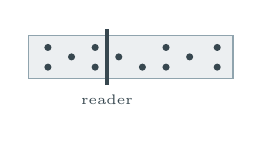
\begin{tikzpicture}
  \draw[draw=nLine, fill=nFill] (0,0) rectangle (2.6,0.55);
  \foreach \x/\y in {0.25/0.15,0.25/0.4,0.55/0.28,0.85/0.15,0.85/0.4,1.15/0.28,1.45/0.15,1.75/0.4,1.75/0.15,2.05/0.28,2.4/0.15,2.4/0.4}
    {\fill[nInk] (\x,\y) circle (0.045);}
  \draw[nInk, very thick] (1.0,-0.08) -- (1.0,0.63);
  \node[font=\tiny, text=nInk, anchor=north] at (1.0,-0.08) {reader};
\end{tikzpicture}}

\newcommand{\diagMemStackSmall}{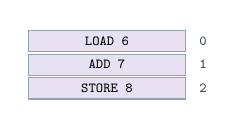
\begin{tikzpicture}
  \node[smallcell, fill=sViolet!18, minimum width=2.0cm] at (0,0.3) {LOAD 6};
  \node[smallcell, fill=sViolet!18, minimum width=2.0cm] at (0,0) {ADD 7};
  \node[smallcell, fill=sViolet!18, minimum width=2.0cm] at (0,-0.3) {STORE 8};
  \node[addr, font=\ttfamily\tiny, anchor=west] at (1.05,0.3) {0};
  \node[addr, font=\ttfamily\tiny, anchor=west] at (1.05,0) {1};
  \node[addr, font=\ttfamily\tiny, anchor=west] at (1.05,-0.3) {2};
\end{tikzpicture}}

\newcommand{\diagTwoMem}{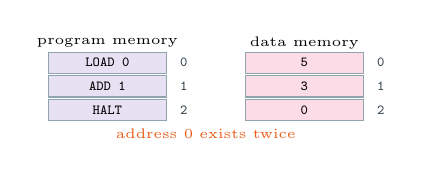
\begin{tikzpicture}
  \node[font=\tiny] at (0,0.55) {program memory};
  \node[font=\tiny] at (2.5,0.55) {data memory};
  \node[smallcell, fill=sViolet!18, minimum width=1.5cm] at (0,0.3) {LOAD 0};
  \node[smallcell, fill=sViolet!18, minimum width=1.5cm] at (0,0) {ADD 1};
  \node[smallcell, fill=sViolet!18, minimum width=1.5cm] at (0,-0.3) {HALT};
  \node[smallcell, fill=sPink!18, minimum width=1.5cm] at (2.5,0.3) {5};
  \node[smallcell, fill=sPink!18, minimum width=1.5cm] at (2.5,0) {3};
  \node[smallcell, fill=sPink!18, minimum width=1.5cm] at (2.5,-0.3) {0};
  \foreach \i in {0,1,2} {
    \node[addr, font=\ttfamily\tiny, anchor=west] at (0.8,{0.3-0.3*\i}) {\i};
    \node[addr, font=\ttfamily\tiny, anchor=west] at (3.3,{0.3-0.3*\i}) {\i};
  }
  \node[font=\tiny, text=AccentOrange] at (1.25,-0.6) {address 0 exists twice};
\end{tikzpicture}}

\newcommand{\diagOneMem}{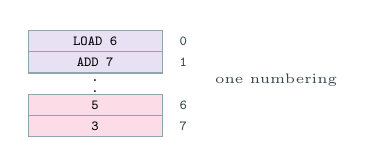
\begin{tikzpicture}
  \node[smallcell, fill=sViolet!18, minimum width=1.7cm] (o0) at (0,0.5) {LOAD 6};
  \node[smallcell, fill=sViolet!18, minimum width=1.7cm] at (0,0.23) {ADD 7};
  \node[smallcell, draw=none, minimum width=1.7cm] at (0,-0.04) {$\vdots$};
  \node[smallcell, fill=sPink!18, minimum width=1.7cm] at (0,-0.31) {5};
  \node[smallcell, fill=sPink!18, minimum width=1.7cm] at (0,-0.58) {3};
  \node[addr, font=\ttfamily\tiny, anchor=west] at (0.95,0.5) {0};
  \node[addr, font=\ttfamily\tiny, anchor=west] at (0.95,0.23) {1};
  \node[addr, font=\ttfamily\tiny, anchor=west] at (0.95,-0.31) {6};
  \node[addr, font=\ttfamily\tiny, anchor=west] at (0.95,-0.58) {7};
  \node[font=\tiny, text=nInk, anchor=west] at (1.4,0) {one numbering};
\end{tikzpicture}}

\newcommand{\diagDecimal}{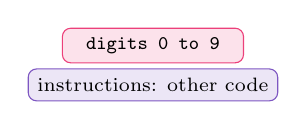
\begin{tikzpicture}
  \node[draw=sPink, fill=sPink!15, rounded corners=3pt, font=\ttfamily\scriptsize, minimum height=0.4cm,
    minimum width=2.3cm] at (0,0.28) {digits 0 to 9};
  \node[draw=sViolet, fill=sViolet!15, rounded corners=3pt, font=\scriptsize, minimum height=0.4cm,
    minimum width=2.3cm] at (0,-0.22) {instructions: other code};
\end{tikzpicture}}

\newcommand{\diagBinary}{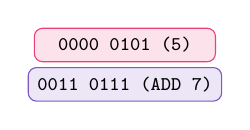
\begin{tikzpicture}
  \node[draw=sPink, fill=sPink!15, rounded corners=3pt, font=\ttfamily\scriptsize, minimum height=0.4cm,
    minimum width=2.3cm] at (0,0.28) {0000 0101 (5)};
  \node[draw=sViolet, fill=sViolet!15, rounded corners=3pt, font=\ttfamily\scriptsize, minimum height=0.4cm,
    minimum width=2.3cm] at (0,-0.22) {0011 0111 (ADD 7)};
\end{tikzpicture}}

\newcommand{\diagParallel}{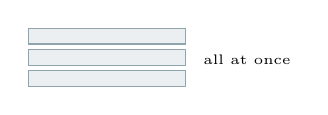
\begin{tikzpicture}
  \foreach \k in {0,1,2} {\draw[fill=nFill, draw=nLine] (0,{0.6-0.27*\k}) rectangle (2.0,{0.4-0.27*\k});}
  \node[font=\tiny, anchor=west] at (2.1,0.2) {all at once};
\end{tikzpicture}}

\newcommand{\diagDataflow}{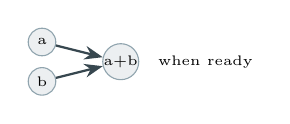
\begin{tikzpicture}[>=Stealth]
  \node[circle, draw=nLine, fill=nFill, minimum size=0.35cm, inner sep=0pt, font=\tiny] (a) at (0,0.3) {a};
  \node[circle, draw=nLine, fill=nFill, minimum size=0.35cm, inner sep=0pt, font=\tiny] (b) at (0,-0.2) {b};
  \node[circle, draw=nLine, fill=nFill, minimum size=0.4cm, inner sep=0pt, font=\tiny] (c) at (1.0,0.05) {a+b};
  \draw[->, thick, nInk] (a) -- (c); \draw[->, thick, nInk] (b) -- (c);
  \node[font=\tiny, anchor=west] at (1.35,0.05) {when ready};
\end{tikzpicture}}

\newcommand{\diagSequential}{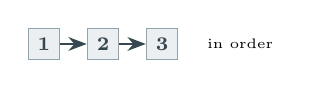
\begin{tikzpicture}[>=Stealth]
  \foreach \k in {1,2,3} {\node[draw=nLine, fill=nFill, text=nInk, minimum size=0.4cm, inner sep=0pt, font=\scriptsize\bfseries]
    (s\k) at ({0.75*\k-0.75},0.05) {\k};}
  \draw[->, thick, nInk] (s1) -- (s2); \draw[->, thick, nInk] (s2) -- (s3);
  \node[font=\tiny, anchor=west] at (1.95,0.05) {in order};
\end{tikzpicture}}

\newcommand{\diagMonolith}{
\begin{tikzpicture}
  \node[draw=nLine, very thick, rounded corners=4pt, fill=nFill, text=nInk, minimum width=2.6cm, minimum height=0.85cm,
    font=\scriptsize, align=center] {one block:\\[-1pt]everything mixed together};
\end{tikzpicture}}

\newcommand{\diagUnits}{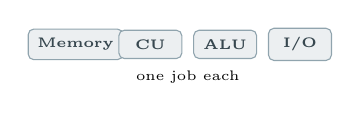
\begin{tikzpicture}
  \node[draw=nLine, fill=nFill, text=nInk, rounded corners=2pt, font=\tiny\bfseries, minimum width=0.8cm, minimum height=0.36cm] at (0,0.22) {Memory};
  \node[draw=nLine, fill=nFill, text=nInk, rounded corners=2pt, font=\tiny\bfseries, minimum width=0.8cm, minimum height=0.36cm] at (0.95,0.22) {CU};
  \node[draw=nLine, fill=nFill, text=nInk, rounded corners=2pt, font=\tiny\bfseries, minimum width=0.8cm, minimum height=0.36cm] at (1.9,0.22) {ALU};
  \node[draw=nLine, fill=nFill, text=nInk, rounded corners=2pt, font=\tiny\bfseries, minimum width=0.8cm, minimum height=0.36cm] at (2.85,0.22) {I/O};
  \node[font=\tiny] at (1.425,-0.2) {one job each};
\end{tikzpicture}}

% ---------- helpers for the CPU section ----------
\tikzset{
  reg/.style={draw=nLine, very thick, fill=white, text=nInk, rounded corners=2pt,
    minimum width=1.95cm, minimum height=0.55cm, inner sep=2pt, font=\ttfamily\scriptsize, align=center},
  cpuunit/.style={very thick, rounded corners=3pt, minimum width=1.2cm, minimum height=0.6cm,
    inner sep=2pt, font=\scriptsize\bfseries, align=center},
  hot/.style={aexec, label={[text=aExec, inner sep=1pt, font=\tiny]right:$\blacktriangleleft$}},
  hotdata/.style={aread},
  hotwrite/.style={awrite},
  hotalu/.style={aexec},
  fetcharrow/.style={-{Stealth}, very thick, nInk, rounded corners=3pt},
  dataarrow/.style={-{Stealth}, very thick, nInk, rounded corners=3pt},
  steplabel/.style={font=\tiny\bfseries, fill=white, inner sep=1pt},
}
% memory with the running example
% #1 highlighted instruction (0-3, -1 = none)  #2 text of cell 8  #3 highlighted data cell (6-8, 0 = none)
\newcommand{\mempanel}[3]{%
  \node[font=\scriptsize\bfseries, text=nInk] at (0,1.8) {Memory};
  \foreach \i/\t in {0/{0001 0110\ \ LOAD 6},1/{0011 0111\ \ ADD 7},2/{0010 1000\ \ STORE 8},3/{0111 0000\ \ HALT}} {
    \ifnum\i=#1
      \node[instrcell, minimum width=2.9cm, hot] (m\i) at (0,{1.35-0.45*\i}) {\t};
    \else
      \node[instrcell, minimum width=2.9cm] (m\i) at (0,{1.35-0.45*\i}) {\t};
    \fi
    \node[addr, anchor=east] at (-1.5,{1.35-0.45*\i}) {\i};
  }
  \node[memcell, draw=none, minimum width=2.9cm] at (0,-0.45) {$\vdots$};
  \foreach \i/\t/\y in {6/{0000 0101\ \ (5)}/-0.9,7/{0000 0011\ \ (3)}/-1.35,8/{#2}/-1.8} {
    \ifnum\i=#3
      \ifnum\i=8 \node[datacell, minimum width=2.9cm, hotwrite] (m\i) at (0,\y) {\t};\else \node[datacell, minimum width=2.9cm, hotdata] (m\i) at (0,\y) {\t};\fi
    \else
      \node[datacell, minimum width=2.9cm] (m\i) at (0,\y) {\t};
    \fi
    \node[addr, anchor=east] at (-1.5,\y) {\i};
  }
}
% the CPU, built up step by step
% #1 level: 0 empty, 1 +PC, 2 +IR, 3 +AC, 4 +ALU, 5 +CU   #2 PC   #3 IR   #4 AC   #5 extra ALU style
\newcommand{\cpupanel}[5]{%
  \node[draw=nLine, very thick, rounded corners=6pt, fill=nFill!50, minimum width=4.65cm,
    minimum height=3.85cm, anchor=west] (cpu) at (2.45,-0.2) {};
  \node[font=\scriptsize\bfseries, text=nInk, anchor=north west] at ([shift={(0.1,-0.06)}]cpu.north west) {CPU};
  \ifnum#1>0 \node[reg] (pc) at (3.65,0.95) {\textbf{PC}\ \ #2}; \fi
  \ifnum#1>1 \node[reg] (ir) at (3.65,0.0) {\textbf{IR}\\[-1pt]#3}; \fi
  \ifnum#1>2 \node[reg] (ac) at (3.65,-1.05) {\textbf{AC}\ \ #4}; \fi
  \ifnum#1>3 \node[cpuunit, draw=nLine, fill=nFill, text=nInk, #5] (alu) at (6.3,-1.05)
    {\faCalculator\\[-1pt]ALU}; \fi
  \ifnum#1>4 \node[cpuunit, draw=nLine, fill=nFill, text=nInk] (cu) at (6.3,0.5)
    {\faCogs\\[-1pt]CU}; \fi
}
% explanation slide: #1 title, #2 tikz body (memory + CPU), #3 right-hand column
\newcommand{\explainframe}[3]{%
\begin{frame}{#1}
  \begin{columns}[c,onlytextwidth]
    \column{0.58\textwidth}
      \centering
      \begin{tikzpicture}[>=Stealth, scale=0.92, every node/.append style={transform shape}]
        #2
      \end{tikzpicture}
    \column{0.4\textwidth}
      #3
  \end{columns}
\end{frame}}
% boxes for the right-hand column
\newcommand{\defbox}[1]{%
  \begin{beamercolorbox}[rounded=true,sep=0.1cm,wd=\linewidth]{block body example}
    \footnotesize #1
  \end{beamercolorbox}\vspace{0.06cm}}
\newcommand{\stepbox}[2]{%
  \begin{beamercolorbox}[rounded=true,sep=0.09cm,wd=\linewidth]{block body}
    \footnotesize\textbf{#1}\\ #2
  \end{beamercolorbox}\vspace{0.06cm}}
\newcommand{\phasename}[1]{%
  {\centering\footnotesize Name of this phase:\ \colorbox{DeepBlue}{\textcolor{white}{\textbf{#1}}}\par}}
% small tag above the CPU box: which instruction is being executed
\newcommand{\executing}[1]{%
  \node[font=\scriptsize\bfseries, text=AccentOrange, anchor=south east] at ([yshift=1pt]cpu.north east)
    {Executing: \texttt{#1}};}
\newcommand{\statebox}[1]{%
  {\centering\scriptsize\textcolor{DeepBlue}{\textbf{State:}}\ #1\par}}

\lstset{
  language=Python,
  basicstyle=\color{VSText}\ttfamily\footnotesize,
  keywordstyle=\color{VSPurple}\bfseries,
  stringstyle=\color{VSString},
  commentstyle=\color{VSComment}\itshape,
  numbers=left,
  numberstyle=\tiny\color{gray},
  stepnumber=1,
  breaklines=true,
  showstringspaces=false,
  xleftmargin=15pt,
  xrightmargin=5pt,
  frame=none
}

% MARIE assembly: line numbers start at 0, so a line number equals the memory address
\lstdefinelanguage{MARIE}{
  morekeywords={Load,Store,Add,Subt,Input,Output,Halt,Jump,Skipcond,Clear,DEC},
  sensitive=false,
  comment=[l]{/},
}
\lstdefinestyle{marie}{language=MARIE, firstnumber=0, basicstyle=\color{VSText}\ttfamily\scriptsize,
  keywordstyle=\color{VSBlue}\bfseries, commentstyle=\color{VSComment}\itshape,
  columns=fixed, basewidth=0.52em, keepspaces=true, breaklines=false, xleftmargin=12pt}

\BeforeBeginEnvironment{lstlisting}{%
  \begin{beamercolorbox}[rounded=true,sep=2mm,wd=\linewidth]{vscodelisting}%
  
\begin{tikzpicture}
    \fill[nLine] (0,0) circle (3pt);
    \fill[nLine] (0.35,0) circle (3pt);
    \fill[nLine] (0.70,0) circle (3pt);
  \end{tikzpicture}%
  \vspace{-0.2cm}%
}
\AfterEndEnvironment{lstlisting}{\end{beamercolorbox}}

\title{Computer Hardware}
\subtitle{Introduction to Processor Architecture}
\author{Ksawery Możdżyński}
\date{}

\begin{document}

\begin{frame}
  \titlepage
\end{frame}

\begin{frame}{Agenda For Today}
  \Large
  \begin{itemize}
    \item[\textcolor{DeepBlue}{\faLaptop}] \textbf{1. What Is a Computer?} \\
    \textcolor{gray}{\small Input, programs, processing, output, and programmability}
    \vspace{0.25cm}

    \item[\textcolor{DeepBlue}{\faCogs}] \textbf{2. Designing a Computer} \\
    \textcolor{gray}{\small Five design decisions behind the von Neumann model}
    \vspace{0.25cm}

    \item[\textcolor{DeepBlue}{\faMicrochip}] \textbf{3. How Does a CPU Work?} \\
    \textcolor{gray}{\small Processor functions, registers, ALU, CU, and the instruction cycle}
    \vspace{0.25cm}

    \item[\textcolor{DeepBlue}{\faLaptop}] \textbf{4. Programming a Simple CPU} \\
    \textcolor{gray}{\small MARIE.js, assembly instructions, input/output, jumps, and loops}
  \end{itemize}
\end{frame}

\section{What is a computer?}

\begin{frame}
  \begin{beamercolorbox}[rounded=true,sep=0.25cm,wd=\textwidth]{block title}
    \centering\large Formal definition
  \end{beamercolorbox}
  \begin{beamercolorbox}[rounded=true,sep=0.25cm,wd=\textwidth]{block body}
    \centering\small
    A computer is a \textbf{programmable} device that accepts
    \textcolor{sPinkText}{\textbf{data}} \textbf{as input},
    processes it according to \textcolor{sViolet}{\textbf{a set of instructions (a program)}},
    and \textbf{produces output}.
    It usually also \textbf{stores data and results}.
  \end{beamercolorbox}

  \vspace{0.25cm}
  \begin{center}
    \begin{tikzpicture}[
      >=Stealth,
      role/.style={very thick, rounded corners=5pt, minimum width=3.0cm,
        minimum height=1.05cm, align=center, font=\bfseries, drop shadow},
      core/.style={draw=nInk, very thick, rounded corners=8pt, fill=nInk,
        text=white, minimum width=3.7cm, minimum height=1.9cm, align=center,
        font=\Large\bfseries, drop shadow},
      arrow/.style={-{Stealth}, very thick}
    ]
      \node[core] (computer) at (4,0) {\faMicrochip\\[-2pt]\normalsize COMPUTER};

      \node[role, draw=sPink, fill=sPink!15] (input) at (-0.95,0.7)
        {\textcolor{sPinkText}{\faDownload}\ Input\\[-2pt]\scriptsize data enters};
      \node[role, draw=sViolet, fill=sViolet!15] (program) at (-0.95,-0.7)
        {\textcolor{sViolet}{\faCode}\ Program\\[-2pt]\scriptsize instructions};
      \node[role, draw=nLine, fill=nFill, text=nInk, above=0.6cm of computer] (storage)
        {\faDatabase\ Storage\\[-2pt]\scriptsize data and results};
      \node[role, draw=nLine, fill=nFill, text=nInk, right=1.6cm of computer] (output)
        {\faUpload\ Output\\[-2pt]\scriptsize results};

      \draw[arrow, nInk]  (input.east)   -- (computer.west |- input.east);
      \draw[arrow, nInk] (program.east) -- (computer.west |- program.east);
      \draw[arrow, nInk]       (computer.east) -- (output.west);
      \draw[arrow, nInk, <->] (computer.north) -- (storage.south);
    \end{tikzpicture}
  \end{center}
\end{frame}

\begin{frame}
  \begin{beamercolorbox}[rounded=true,sep=0.25cm,wd=\textwidth]{block title}
    \centering\large The central idea: programmability
  \end{beamercolorbox}
  \begin{beamercolorbox}[rounded=true,sep=0.25cm,wd=\textwidth]{block body}
    \centering\small
    Programmability means that the same hardware can perform different tasks:
    given the \textcolor{sPinkText}{\textbf{same data}}, different
    \textcolor{sViolet}{\textbf{programs}} make the computer produce different
    \textbf{results}.
  \end{beamercolorbox}

  \vspace{0.3cm}
  \begin{center}
    \begin{tikzpicture}[
      >=Stealth,
      data/.style={draw=sPink, very thick, rounded corners=5pt, fill=sPink!15,
        minimum width=2.9cm, minimum height=0.95cm, align=center, font=\bfseries, drop shadow},
      program/.style={draw=sViolet, very thick, rounded corners=5pt, fill=sViolet!15,
        minimum width=2.9cm, minimum height=0.95cm, align=center, font=\bfseries, drop shadow},
      computer/.style={draw=nInk, very thick, rounded corners=8pt, fill=nInk,
        text=white, minimum width=3.6cm, minimum height=0.95cm, align=center,
        font=\bfseries, drop shadow},
      result/.style={draw=nLine, very thick, rounded corners=5pt, fill=nFill, text=nInk,
        minimum width=2.9cm, minimum height=0.95cm, align=center, font=\bfseries, drop shadow},
      arrow/.style={-{Stealth}, very thick}
    ]
      % ---------- LEFT: Program 1 ----------
      \node[data]     (d1) at (-4.85, 0)   {\textcolor{sPinkText}{\faDatabase}\ Same data\\[-2pt]\scriptsize\texttt{x = 5}};
      \node[program]  (p1) at (-1.75, 0)   {\textcolor{sViolet}{\faCode}\ Program 1\\[-2pt]\scriptsize\texttt{result = x * 2}};
      \node[computer] (c1) at (-3.3, -1.5) {\faMicrochip\ SAME COMPUTER};
      \node[result]   (r1) at (-3.3, -3.0) {\faCheckCircle\ Output 1\\[-2pt]\scriptsize\texttt{10}};

      \draw[arrow, nInk]  (d1.south) -- (d1.south |- c1.north);
      \draw[arrow, nInk] (p1.south) -- (p1.south |- c1.north);
      \draw[arrow, nInk]       (c1.south) -- (r1.north);

      % ---------- RIGHT: Program 2 ----------
      \node[data]     (d2) at (1.75, 0)   {\textcolor{sPinkText}{\faDatabase}\ Same data\\[-2pt]\scriptsize\texttt{x = 5}};
      \node[program]  (p2) at (4.85, 0)   {\textcolor{sViolet}{\faCode}\ Program 2\\[-2pt]\scriptsize\texttt{result = x + 4}};
      \node[computer] (c2) at (3.3, -1.5) {\faMicrochip\ SAME COMPUTER};
      \node[result]   (r2) at (3.3, -3.0) {\faCheckCircle\ Output 2\\[-2pt]\scriptsize\texttt{9}};

      \draw[arrow, nInk]  (d2.south) -- (d2.south |- c2.north);
      \draw[arrow, nInk] (p2.south) -- (p2.south |- c2.north);
      \draw[arrow, nInk]       (c2.south) -- (r2.north);

      % ---------- divider ----------
      \draw[nLine, dashed, thick] (0,0.7) -- (0,-3.5);
    \end{tikzpicture}
  \end{center}
\end{frame}

% =====================================================================
%  VON NEUMANN SECTION (reworked)
% =====================================================================

\section{Designing a computer}

% ---------- 1. The definition is too general ----------
\begin{frame}{Is this definition precise enough?}
  \begin{beamercolorbox}[rounded=true,sep=0.18cm,wd=\textwidth]{block body}
    \centering\small
    ``A programmable device that takes input, processes it according to a program, and produces output''
    tells us \textbf{what a computer does}, but not \textbf{how it is organised}.
  \end{beamercolorbox}
  \vspace{0.2cm}
  \begin{center}
    \footnotesize
    \renewcommand{\arraystretch}{1.25}
    \begin{tabular}{cp{4.9cm}p{7.9cm}}
      \toprule
      & \textbf{Design dilemma} & \textbf{Possible answers} \\
      \midrule
      \num{1} & Where does the program live? & Wired program; Program on tape; Program in memory \\
      \num{2} & Do instructions and data live in the same place? & Two separate memories; One shared memory \\
      \num{3} & How do we represent information? & Decimal numbers, special codes; Everything as binary numbers \\
      \num{4} & What runs next? & Many at once; When the data is ready; One after another \\
      \num{5} & How is the machine organised? & One undivided machine; Separate units \\
      \bottomrule
    \end{tabular}
  \end{center}
  \begin{alertblock}{We need a more precise model}
    \centering\small
    Different answers give different computers.
  \end{alertblock}
\end{frame}

\begin{frame}{Let's design our own computer model}
  \begin{beamercolorbox}[rounded=true,sep=0.25cm,wd=\textwidth]{block title}
    \centering\large A computer architect's perspective
  \end{beamercolorbox}
  \begin{beamercolorbox}[rounded=true,sep=0.25cm,wd=\textwidth]{block body}
    \centering\small
    Before looking at the final model, let us step into the role of a computer architect
    and make the key design decisions.
  \end{beamercolorbox}

  \vfill
  \begin{alertblock}{Our approach}
    \centering\small
    We will analyse the design choices embodied in the von Neumann model.
  \end{alertblock}
\end{frame}

% =====================================================================
%  VON NEUMANN SECTION: five design dilemmas and von Neumann's decisions
% =====================================================================

% ===================== DILEMMA 1: where is the program? =====================
\begin{frame}{Dilemma 1: where does the program live?}
  \begin{beamercolorbox}[rounded=true,sep=0.16cm,wd=\textwidth]{block body}
    \centering\small
    \textbf{Design question:} how can one machine run many different programs without being rebuilt each time?
  \end{beamercolorbox}
  \vspace{0.2cm}
  \begin{columns}[T,onlytextwidth]
    \column{0.31\textwidth}
      \optcard{Wired program}{\diagWired}
        {very fast and highly optimised for one fixed task}
        {a new task means physical rewiring}
    \column{0.31\textwidth}
      \optcard{Program on tape}{\diagTape}
        {swap the tape to change the task}
        {slow mechanical reading; loops and jumps are awkward}
    \column{0.31\textwidth}
      \optcard{Program in memory}{\diagMemStackSmall}
        {fast electronic access to any instruction}
        {needs enough memory and a way to load the program}
  \end{columns}
  \vfill
  {\centering\small\textcolor{DeepBlue}{\textbf{Which would you choose, and why?}}\par}
  \vspace{0.05cm}
  \progress{0}
\end{frame}

\begin{frame}{Decision 1: keep the program in memory}
  \begin{beamercolorbox}[rounded=true,sep=0.16cm,wd=\textwidth]{block body}
    \centering\small
    \textbf{Von Neumann's answer:} the program is stored in the computer's \textbf{memory}, as numbered instructions.
  \end{beamercolorbox}
  \vspace{0.05cm}
  \begin{columns}[T,onlytextwidth]
    \column{0.42\textwidth}
      \centering
      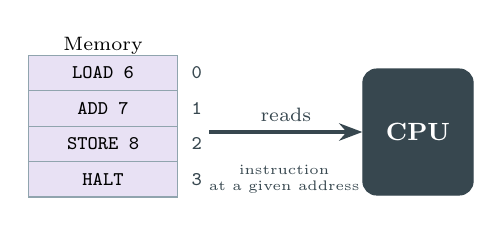
\begin{tikzpicture}[>=Stealth]
        \node[font=\scriptsize] at (0,0.65) {Memory};
        \foreach \i/\t in {0/{LOAD 6},1/{ADD 7},2/{STORE 8},3/{HALT}} {
          \node[instrcell, minimum width=1.9cm] (m\i) at (0,{0.3-0.45*\i}) {\t};
          \node[addr, anchor=west] at (1.0,{0.3-0.45*\i}) {\i};
        }
        \node[draw=nInk, fill=nInk, text=white, rounded corners=5pt, minimum width=1.4cm, minimum height=1.6cm,
          font=\bfseries\small] (cpu) at (4.0,-0.45) {CPU};
        \draw[-{Stealth}, very thick, nInk] (1.35,-0.45) -- node[above, font=\scriptsize] {reads} (cpu.west);
        \node[font=\tiny, text=nInk, align=center] at (2.3,-1.05) {instruction\\at a given address};
      \end{tikzpicture}
    \column{0.55\textwidth}
      \begin{beamercolorbox}[rounded=true,sep=0.13cm,wd=\linewidth]{block body example}
        \footnotesize
        \textbf{What it gives us}
        \begin{itemize}\setlength{\itemsep}{1pt}
          \item One machine, many programs: a new task means new contents of memory.
          \item Any instruction is reachable by its address, so jumps and loops are easy.
        \end{itemize}
      \end{beamercolorbox}
      \vspace{0.08cm}
      \begin{beamercolorbox}[rounded=true,sep=0.13cm,wd=\linewidth]{block body}
        \footnotesize
        \textbf{What it costs:} enough memory, and a way to load the program into it.
      \end{beamercolorbox}
  \end{columns}
  \vfill
  \begin{beamercolorbox}[rounded=true,sep=0.1cm,wd=\textwidth]{block body}
    \centering\footnotesize
    The program is now stored. Next question: where are the data stored?
  \end{beamercolorbox}
  \vspace{0.1cm}
  \progress{1}
\end{frame}

\begin{frame}{Dilemma 2: where do instructions and data live?}
  \begin{beamercolorbox}[rounded=true,sep=0.16cm,wd=\textwidth]{block body}
    \centering\small
    \textbf{Design question:} should instructions and data use the same memory,
    or should they have separate memories?
  \end{beamercolorbox}
  \vspace{0.2cm}
  \begin{columns}[T,onlytextwidth]
    \column{0.46\textwidth}
      \optcard{Separate memories}{\diagTwoMem}
        {instructions and data can be accessed independently}
        {two memories, two address spaces, and more complex organisation}
    \column{0.46\textwidth}
      \optcard{One shared memory}{\diagOneMem}
        {one address space and one simple memory model}
        {instructions and data compete for the same path}
  \end{columns}
  \vfill
  {\centering\small\textcolor{DeepBlue}{\textbf{Which design would you choose, and why?}}\par}
  \vspace{0.05cm}
  \progress{1}
\end{frame}

\begin{frame}{Decision 2: one memory for instructions and data}
  \begin{beamercolorbox}[rounded=true,sep=0.16cm,wd=\textwidth]{block body}
    \centering\small
    \textbf{Von Neumann's answer:} there is \textbf{one memory}. Instructions and data are stored side by side
    and share \textbf{one numbering of cells} (one address space).
  \end{beamercolorbox}
  \vspace{0.1cm}
  \begin{columns}[T,onlytextwidth]
    \column{0.40\textwidth}
      \centering
      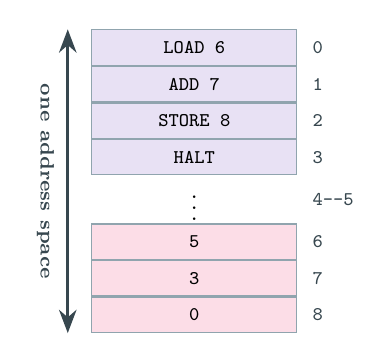
\begin{tikzpicture}[>=Stealth]
        \node[instrcell] (a0) at (0,0) {LOAD 6};
        \node[instrcell, below=0pt of a0] (a1) {ADD 7};
        \node[instrcell, below=0pt of a1] (a2) {STORE 8};
        \node[instrcell, below=0pt of a2] (a3) {HALT};
        \node[memcell, draw=none, below=0pt of a3] (a4) {$\vdots$};
        \node[datacell, below=0pt of a4] (a6) {5};
        \node[datacell, below=0pt of a6] (a7) {3};
        \node[datacell, below=0pt of a7] (a8) {0};
        \node[addr, anchor=west] at ([xshift=2pt]a0.east) {0};
        \node[addr, anchor=west] at ([xshift=2pt]a1.east) {1};
        \node[addr, anchor=west] at ([xshift=2pt]a2.east) {2};
        \node[addr, anchor=west] at ([xshift=2pt]a3.east) {3};
        \node[addr, anchor=west] at ([xshift=2pt]a4.east) {4--5};
        \node[addr, anchor=west] at ([xshift=2pt]a6.east) {6};
        \node[addr, anchor=west] at ([xshift=2pt]a7.east) {7};
        \node[addr, anchor=west] at ([xshift=2pt]a8.east) {8};
        \draw[<->, very thick, nInk] ([xshift=-0.3cm]a0.north west) -- ([xshift=-0.3cm]a8.south west)
          node[midway, below=1pt, sloped, font=\scriptsize\bfseries] {one address space};
      \end{tikzpicture}\\[0.05cm]
      \scriptsize
      \textcolor{sViolet}{$\blacksquare$} instruction\quad\textcolor{sPink}{$\blacksquare$} data
    \column{0.57\textwidth}
      \small
      \textbf{What does ``the same'' mean? Three things:}
      \vspace{0.1cm}
      \begin{itemize}\setlength{\itemsep}{3pt}
        \item \textbf{Same storage.} One memory, not a program memory plus a separate data memory.
        \item \textbf{Same addresses.} One numbering $0,1,2,\dots$; each address belongs to exactly one cell.
        \item \textbf{Same kind of cell.} A cell is a group of bits. There is no special kind of cell for instructions.
      \end{itemize}
      \vspace{0.05cm}
      \footnotesize
      \textcolor{DeepBlue}{\textbf{The price:}} instructions and data travel over the same path (the von Neumann bottleneck, later).
  \end{columns}
  \vfill
  \progress{2}
\end{frame}

\begin{frame}{Decision 2 (continued): how do bits get their meaning?}
  \begin{beamercolorbox}[rounded=true,sep=0.16cm,wd=\textwidth]{block body}
    \centering\small
    Looking at memory alone, we see addresses and bit patterns, not labels such as ``instruction'' or ``data''.
    \textbf{The program context gives the bits their meaning.}
  \end{beamercolorbox}
  \vspace{0.15cm}
  \begin{center}
    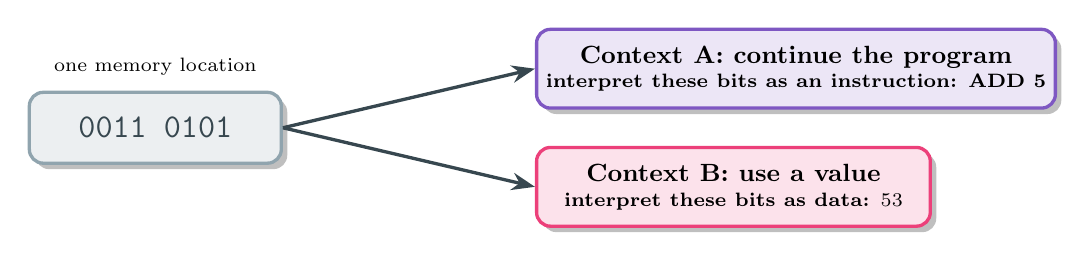
\begin{tikzpicture}[>=Stealth,
      bits/.style={draw=nLine, very thick, rounded corners=5pt, fill=nFill, text=nInk,
        minimum width=3.2cm, minimum height=0.9cm, align=center, font=\ttfamily\large, drop shadow},
      context/.style={draw=nLine, very thick, rounded corners=5pt, minimum width=5.0cm,
        minimum height=1.0cm, align=center, font=\small\bfseries, drop shadow},
      arrow/.style={-{Stealth}, very thick, nInk}]
      \node[bits] (cell) at (0,0) {0011 0101};
      \node[above=2pt of cell, font=\scriptsize] {one memory location};
      \node[context, draw=sViolet, fill=sViolet!15, right=3.2cm of cell, yshift=0.75cm] (instruction)
        {Context A: continue the program\\[-2pt]\scriptsize interpret these bits as an instruction: ADD 5};
      \node[context, draw=sPink, fill=sPink!15, right=3.2cm of cell, yshift=-0.75cm] (data)
        {Context B: use a value\\[-2pt]\scriptsize interpret these bits as data: $53$};
      \draw[arrow] (cell.east) -- (instruction.west);
      \draw[arrow] (cell.east) -- (data.west);
    \end{tikzpicture}
  \end{center}
  \vspace{0.05cm}
  \begin{columns}[T,onlytextwidth]
    \column{0.47\textwidth}
      \begin{beamercolorbox}[rounded=true,sep=0.12cm,wd=\linewidth]{block body example}
        \scriptsize
        \textbf{Key idea:} memory stores bit patterns. It does not store their meaning as a label.
      \end{beamercolorbox}
    \column{0.47\textwidth}
      \begin{beamercolorbox}[rounded=true,sep=0.12cm,wd=\linewidth]{block body}
        \scriptsize
        \textbf{Important:} the same kind of memory cell can hold an instruction or a value, depending on the program context.
      \end{beamercolorbox}
  \end{columns}
  \vfill
  \progress{2}
\end{frame}

% ===================== DILEMMA 3: representation =====================
\begin{frame}{Dilemma 3: how do we represent information?}
  \begin{beamercolorbox}[rounded=true,sep=0.16cm,wd=\textwidth]{block body}
    \centering\small
    \textbf{Design question:} in what form are numbers and instructions kept inside the machine?
  \end{beamercolorbox}
  \vspace{0.2cm}
  \begin{columns}[T,onlytextwidth]
    \column{0.46\textwidth}
      \optcard{Decimal numbers, special codes}{\diagDecimal}
        {close to how people write numbers (early machines such as ENIAC worked in decimal)}
        {more complex circuits (ten states per digit); numbers and instructions need different formats}
    \column{0.46\textwidth}
      \optcard{Everything as binary numbers}{\diagBinary}
        {two-state circuits are simple and reliable; instructions and data share one format}
        {people must convert; long strings of bits}
  \end{columns}
  \vfill
  {\centering\small\textcolor{DeepBlue}{\textbf{Which would you choose, and why?}}\par}
  \vspace{0.05cm}
  \progress{2}
\end{frame}

\begin{frame}{Decision 3: everything is binary}
  \begin{beamercolorbox}[rounded=true,sep=0.14cm,wd=\textwidth]{block body}
    \centering\small
    \textbf{Von Neumann's answer:} both instructions and data are \textbf{binary numbers}: fixed-size groups of bits.
  \end{beamercolorbox}
  \vspace{0.05cm}
  \begin{columns}[T,onlytextwidth]
    \column{0.44\textwidth}
      \centering
      \footnotesize\textbf{An instruction is a number too}\\[0.1cm]
      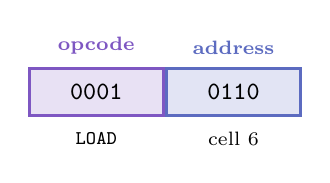
\begin{tikzpicture}[>=Stealth]
        \node[draw=sViolet, fill=sViolet!18, very thick, minimum width=1.7cm, minimum height=0.6cm,
          font=\ttfamily\small] (op) {0001};
        \node[draw=sIndigo, fill=sIndigo!18, very thick, minimum width=1.7cm, minimum height=0.6cm,
          font=\ttfamily\small, right=0pt of op] (ad) {0110};
        \node[above=1pt of op, font=\scriptsize\bfseries, text=sViolet] {opcode};
        \node[above=1pt of ad, font=\scriptsize\bfseries, text=sIndigo] {address};
        \node[below=2pt of op, font=\scriptsize] {\texttt{LOAD}};
        \node[below=2pt of ad, font=\scriptsize] {cell 6};
      \end{tikzpicture}\\[0.12cm]
      \scriptsize
      \begin{tabular}{cc}
        \toprule
        \textbf{Opcode} & \textbf{Operation} \\
        \midrule
        \texttt{0001} & \texttt{LOAD} \\
        \texttt{0010} & \texttt{STORE} \\
        \texttt{0011} & \texttt{ADD} \\
        \texttt{0111} & \texttt{HALT} \\
        \bottomrule
      \end{tabular}
    \column{0.52\textwidth}
      \centering
      \footnotesize\textbf{Our example program, as it sits in memory}\\[0.1cm]
      \scriptsize
      \begin{tabular}{c|c|l}
        \toprule
        \textbf{Address} & \textbf{Bits} & \textbf{Meaning} \\
        \midrule
        0 & \texttt{0001 0110} & \cellcolor{sViolet!15} instruction \texttt{LOAD 6} \\
        1 & \texttt{0011 0111} & \cellcolor{sViolet!15} instruction \texttt{ADD 7} \\
        2 & \texttt{0010 1000} & \cellcolor{sViolet!15} instruction \texttt{STORE 8} \\
        3 & \texttt{0111 0000} & \cellcolor{sViolet!15} instruction \texttt{HALT} \\
        6 & \texttt{0000 0101} & \cellcolor{sPink!15} number 5 \\
        7 & \texttt{0000 0011} & \cellcolor{sPink!15} number 3 \\
        8 & \texttt{0000 0000} & \cellcolor{sPink!15} number 0 (result) \\
        \bottomrule
      \end{tabular}\\[0.1cm]
      \tiny 8-bit teaching format: 4-bit opcode + 4-bit address (opcodes as in MARIE, used later). Real CPUs use longer, richer formats.
  \end{columns}
  \vspace{0.05cm}
  \begin{beamercolorbox}[rounded=true,sep=0.1cm,wd=\textwidth]{block body example}
    \centering\footnotesize
    \textbf{Gain:} one kind of hardware stores, copies and moves both.\quad
    \textbf{Price:} people need tools (assemblers, compilers) to write instructions comfortably.
  \end{beamercolorbox}
  \vfill
  \progress{3}
\end{frame}

% ===================== DILEMMA 4: execution order =====================
\begin{frame}{Dilemma 4: how is instruction execution controlled?}
  \begin{beamercolorbox}[rounded=true,sep=0.16cm,wd=\textwidth]{block body}
    \centering\small
    \textbf{Design question:} should the computer follow the program step by step,
    or can it execute independent operations at the same time?
  \end{beamercolorbox}
  \vspace{0.2cm}
  \begin{columns}[T,onlytextwidth]
    \column{0.31\textwidth}
      \optcard{Parallel execution}{\diagParallel}
        {independent operations can run together}
        {harder to design and coordinate}
    \column{0.31\textwidth}
      \optcard{Data-driven execution}{\diagDataflow}
        {an operation runs when its inputs are ready}
        {complex hardware and less predictable order}
    \column{0.31\textwidth}
      \optcard{Sequential control}{\diagSequential}
        {instructions follow the order of the program}
        {less parallelism at the program level}
  \end{columns}
  \vfill
  {\centering\small\textcolor{DeepBlue}{\textbf{Which would you choose, and why?}}\par}
  \vspace{0.05cm}
  \progress{3}
\end{frame}

\begin{frame}{Decision 4: an ordered program sequence}
  \begin{beamercolorbox}[rounded=true,sep=0.16cm,wd=\textwidth]{block body}
    \centering\small
    \textbf{The von Neumann model:} the program is represented as an \textbf{ordered sequence of instructions}.
    The \textbf{program counter (PC)} remembers the address of the next instruction;
    a jump simply writes a new address into it.
  \end{beamercolorbox}
  \vspace{0.3cm}
  \begin{center}
    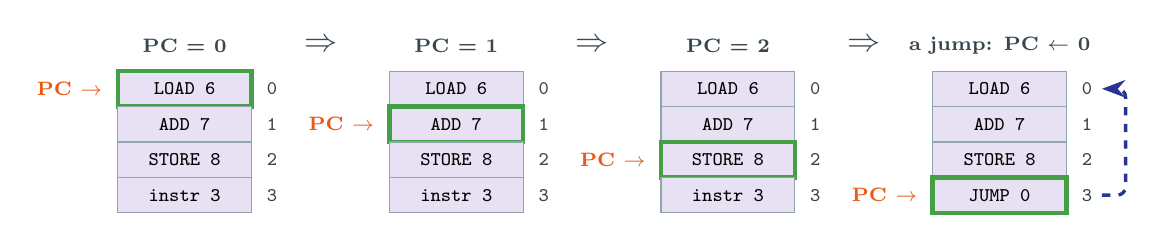
\begin{tikzpicture}[>=Stealth]
      \pcstack{-4.9}{0}{instr 3}{PC = 0}
      \pcstack{-1.45}{1}{instr 3}{PC = 1}
      \pcstack{2.0}{2}{instr 3}{PC = 2}
      \pcstack{5.45}{3}{JUMP 0}{a jump: PC $\leftarrow$ 0}
      \node[font=\large\bfseries, text=nInk] at (-3.17,0.55) {$\Rightarrow$};
      \node[font=\large\bfseries, text=nInk] at (0.28,0.55) {$\Rightarrow$};
      \node[font=\large\bfseries, text=nInk] at (3.73,0.55) {$\Rightarrow$};
      \draw[-{Stealth}, very thick, DeepBlue, dashed, rounded corners=3pt]
        (6.75,-1.35) -- (7.05,-1.35) -- (7.05,0) -- (6.75,0);
    \end{tikzpicture}
  \end{center}
  \vspace{0.05cm}
  \begin{columns}[T,onlytextwidth]
    \column{0.47\textwidth}
      \begin{beamercolorbox}[rounded=true,sep=0.12cm,wd=\linewidth]{block body example}
        \scriptsize
        \textbf{Gain:} a predictable program order. Jumps make loops and conditions possible.
      \end{beamercolorbox}
    \column{0.47\textwidth}
      \begin{beamercolorbox}[rounded=true,sep=0.12cm,wd=\linewidth]{block body}
        \scriptsize
        \textbf{Important:} modern CPUs may overlap independent instructions internally, while preserving the program's visible order.
      \end{beamercolorbox}
  \end{columns}
  \vfill
  \progress{4}
\end{frame}

% ===================== DILEMMA 5: organisation =====================
\begin{frame}{Dilemma 5: how is the machine organised?}
  \begin{beamercolorbox}[rounded=true,sep=0.16cm,wd=\textwidth]{block body}
    \centering\small
    \textbf{Design question:} should the computer be one undivided whole, or a set of parts with separate jobs?
  \end{beamercolorbox}
  \vspace{0.2cm}
  \begin{columns}[T,onlytextwidth]
    \column{0.46\textwidth}
      \optcard{One undivided machine}{\diagMonolith}
        {can be tuned for a single task}
        {hard to understand, change or reuse: every change touches everything}
    \column{0.46\textwidth}
      \optcard{Separate units}{\diagUnits}
        {each part has one clear job and can be designed and improved on its own}
        {the parts must be connected to each other}
  \end{columns}
  \vfill
  {\centering\small\textcolor{DeepBlue}{\textbf{Which would you choose, and why?}}\par}
  \vspace{0.05cm}
  \progress{4}
\end{frame}

\begin{frame}{Decision 5: separate functional units}
  \begin{beamercolorbox}[rounded=true,sep=0.16cm,wd=\textwidth]{block body}
    \centering\small
    \textbf{Von Neumann's answer:} separate functional units for memory, control, computation, registers, and I/O.
  \end{beamercolorbox}
  \vspace{0.05cm}
  \begin{center}
    \begin{tikzpicture}[
      >=Stealth,
      module/.style={draw=nLine, very thick, rounded corners=4pt, align=center, text=nInk,
        font=\small\bfseries, drop shadow, inner sep=2pt},
      external/.style={draw=nLine, very thick, rounded corners=5pt, fill=nFill, text=nInk,
        minimum width=1.6cm, minimum height=0.85cm, align=center, font=\small\bfseries, drop shadow},
      flow/.style={-{Stealth}, very thick, nInk},
      inside/.style={{Stealth[length=1.6mm,width=1.4mm]}-{Stealth[length=1.6mm,width=1.4mm]}, thick, nInk},
      busline/.style={very thick, nLine}
    ]
      % ---------- blocks (all bottoms aligned at y = -1.2) ----------
      \node[module, anchor=south, fill=nFill, minimum width=2.2cm, minimum height=1.5cm] (io) at (-3.6,-1.2)
        {\faArrowRight\ I/O\\[-2pt]\scriptsize interfaces\\[-3pt]\scriptsize to devices};
      \node[module, anchor=south, fill=nFill, minimum width=2.2cm, minimum height=1.5cm] (memory) at (-0.6,-1.2)
        {\faDatabase\ Memory\\[-2pt]\scriptsize program\\[-3pt]\scriptsize + data};

      % CPU: one box that contains control, computation and registers
      \node[draw=nLine, very thick, rounded corners=6pt, fill=nFill!50, minimum width=6.0cm,
        minimum height=2.35cm, anchor=south, drop shadow] (cpu) at (4.0,-1.2) {};
      \node[font=\scriptsize\bfseries, text=nInk, anchor=south west] at ([shift={(0.12,0.08)}]cpu.south west) {CPU};
      \node[module, fill=nFill, minimum width=2.45cm, minimum height=0.78cm] (cu) at (2.55,0.52)
        {\faCogs\ CU\\[-2pt]\scriptsize directs operations};
      \node[module, fill=nFill, minimum width=2.45cm, minimum height=0.78cm] (alu) at (5.45,0.52)
        {\faCalculator\ ALU\\[-2pt]\scriptsize performs calculations};
      \node[module, fill=nFill, minimum width=4.0cm, minimum height=0.72cm] (reg) at (4.0,-0.58)
        {\faStickyNote\ Registers\\[-2pt]\scriptsize fast working values};

      % ---------- outside world ----------
      \node[external] (input) at (-6.45,0.2) {Input\\[-2pt]\scriptsize program/data};
      \node[external] (output) at (-6.45,-0.95) {Output\\[-2pt]\scriptsize results};

      % ---------- system bus ----------
      \node[fill=nLine, minimum width=10.8cm, minimum height=0.22cm, inner sep=0pt] (bus) at (0.55,-1.6) {};
      \node[font=\tiny\bfseries, text=white] at (1.8,-1.6) {SYSTEM BUS};

      % ---------- connections ----------
      % outside world <-> I/O subsystem only
      \draw[flow] (input.east) -- (input.east -| io.west);
      \draw[flow] (io.west |- output.east) -- (output.east);
      % memory, CPU and I/O all share the bus
      \draw[busline] (io.south) -- (io.south |- bus.north);
      \draw[busline] (memory.south) -- (memory.south |- bus.north);
      \draw[busline] (cpu.south) -- (cpu.south |- bus.north);
      % inside the CPU
      \draw[flow] (cu.east) -- (alu.west);
      \draw[inside] (cu.south) -- (cu.south |- reg.north);
      \draw[inside] (alu.south) -- (alu.south |- reg.north);

      % ---------- the whole computer ----------
      \node[draw=nLine, very thick, rounded corners=8pt, inner sep=0.2cm, fit=(io)(memory)(cpu)(bus),
        label={[font=\small\bfseries, text=nInk]above:COMPUTER}] (computer) {};
    \end{tikzpicture}
  \end{center}
  \vspace{0.02cm}
  \begin{beamercolorbox}[rounded=true,sep=0.1cm,wd=\textwidth]{block body example}
    \centering\footnotesize
    Input and output enter through the I/O subsystem; program and data live in Memory; a bus connects the units.
  \end{beamercolorbox}
  \vspace{0.08cm}
  \progress{5}
\end{frame}

% ---------- Student task: explore alternative design choices ----------
\begin{frame}{Task: explore alternative design choices}
  \begin{beamercolorbox}[rounded=true,sep=0.16cm,wd=\textwidth]{block body}
    \centering\small
    \textbf{Choose one design or extension} and investigate why it is useful.
  \end{beamercolorbox}
  \vspace{0.14cm}
  \begin{columns}[T,onlytextwidth]
    \column{0.31\textwidth}
      \begin{beamercolorbox}[rounded=true,sep=0.11cm,wd=\linewidth]{block body example}
        \centering\small\textcolor{nInk}{\large\faDatabase}\\[-1mm]
        \textbf{Memory organisation}\\[0.04cm]
        \raggedright\footnotesize
        \textbf{Harvard architecture}\\
        Separate instruction and data memories.
      \end{beamercolorbox}
    \column{0.31\textwidth}
      \begin{beamercolorbox}[rounded=true,sep=0.11cm,wd=\linewidth]{block body}
        \centering\small\textcolor{nInk}{\large\faCalculator}\\[-1mm]
        \textbf{Data processing}\\[0.04cm]
        \raggedright\footnotesize
        \textbf{SIMD architecture}\\
        One operation applied to many data values.
        Used in graphics and image processing.
      \end{beamercolorbox}
    \column{0.31\textwidth}
      \begin{beamercolorbox}[rounded=true,sep=0.11cm,wd=\linewidth]{block body example}
        \centering\small\textcolor{nInk}{\large\faCogs}\\[-1mm]
        \textbf{Execution control}\\[0.04cm]
        \raggedright\footnotesize
        \textbf{Dataflow architecture}\\
        Operations run when their inputs are ready.
      \end{beamercolorbox}
  \end{columns}

  \vspace{0.08cm}
  \begin{beamercolorbox}[rounded=true,sep=0.08cm,wd=\textwidth]{block title}
    \centering\small\textbf{Compare \ $\rightarrow$\ Explain \ $\rightarrow$\ Evaluate}
  \end{beamercolorbox}
  \begin{columns}[T,onlytextwidth]
    \column{0.31\textwidth}\centering\small
      \textbf{1. Compare}\\[-1mm]
      Which design choice differs from von Neumann?
    \column{0.31\textwidth}\centering\small
      \textbf{2. Explain}\\[-1mm]
      What problem does this design solve, and where is it used?
    \column{0.31\textwidth}\centering\small
      \textbf{3. Evaluate}\\[-1mm]
      What is one advantage and one limitation?
  \end{columns}

\end{frame}

% =====================================================================
%  HOW DOES A CPU WORK?
% =====================================================================
\section{How does a CPU work?}

% ---------- 0. What does a processor do, before any component names ----------
\begin{frame}{What does a processor do?}
  \begin{beamercolorbox}[rounded=true,sep=0.16cm,wd=\textwidth]{block body}
    \centering\small
    A processor is the active part of a computer: it follows instructions and transforms data into results.
  \end{beamercolorbox}
  \vspace{0.15cm}
  \begin{columns}[T,onlytextwidth]
    \column{0.55\textwidth}
      \small
      \num{1}\ \textbf{Read instructions} -- find out what needs to be done.\\[4pt]
      \num{2}\ \textbf{Understand instructions} -- identify the operation.\\[4pt]
      \num{3}\ \textbf{Get data} -- obtain the values needed for it.\\[4pt]
      \num{4}\ \textbf{Perform the operation} -- calculate, compare, transform.\\[4pt]
      \num{5}\ \textbf{Store the result} -- keep it, or send it onward.
    \column{0.4\textwidth}
      \centering
      \resizebox{\linewidth}{!}{%
      \begin{tikzpicture}[>=Stealth,
        proc/.style={draw=nLine, very thick, rounded corners=6pt, fill=nFill, text=nInk,
          minimum width=2.6cm, minimum height=1.4cm, align=center, font=\bfseries, drop shadow},
        io/.style={draw=nLine, very thick, rounded corners=4pt, fill=nFill, text=nInk,
          minimum width=2.1cm, minimum height=0.7cm, align=center, font=\small\bfseries, drop shadow},
        flow/.style={-{Stealth}, very thick, nInk}]
        \node[proc] (p) {PROCESSOR};
        \node[io, above=0.6cm of p] (ins) {\textcolor{sViolet}{\faDownload}\ Instructions};
        \node[io, below=0.6cm of p] (dat) {\textcolor{sPinkText}{\faDownload}\ Data};
        \node[io, right=1.1cm of p] (res) {\faUpload\ Results};
        \draw[flow] (ins) -- (p);
        \draw[flow] (dat) -- (p);
        \draw[flow] (p) -- (res);
      \end{tikzpicture}}
  \end{columns}
  \vfill
  \begin{beamercolorbox}[rounded=true,sep=0.1cm,wd=\textwidth]{block body example}
    \centering\footnotesize
    First understand the jobs. Next, we will meet the hardware parts that perform them.
  \end{beamercolorbox}
\end{frame}

% ---------- 1. Starting point ----------
\explainframe{What does the CPU work with?}
  {\mempanel{-1}{0000 0000\ \ (0)}{0}
   \cpupanel{0}{}{}{}{}
   \node[font=\scriptsize, text=gray, align=center] at (cpu.center) {empty for now};
   \draw[{Stealth}-{Stealth}, very thick, nLine] (1.5,-0.2) -- node[above, font=\scriptsize\bfseries, text=nInk] {bus} (cpu.west |- 0,-0.2);}
  {\footnotesize
   The program and its data are in memory. The CPU is connected to memory by the bus
   and can do only two things with it:\par\vspace{0.1cm}
   \stepbox{Read}{The CPU can \textbf{read one cell} from memory.}
   \stepbox{Write}{The CPU can \textbf{write to one cell} in memory.}
   \begin{beamercolorbox}[rounded=true,sep=0.1cm,wd=\linewidth]{block body example}
     \footnotesize\centering
     The CPU does \textbf{not} see the whole program.\\ At any moment it gets \textbf{only one cell}.
   \end{beamercolorbox}}

% ---------- 2. Which cell to read? PC ----------
\explainframe{The program counter (PC)}
  {\mempanel{-1}{0000 0000\ \ (0)}{0}
   \cpupanel{1}{0}{}{}{}
   \executing{LOAD 6}
   \draw[-{Stealth}, thick, dashed, orange!80!black, rounded corners=3pt] (pc.west) -- ++(-0.45,0) |- (m0.east);
   \node[font=\tiny, text=orange!80!black, align=center, anchor=north] at (pc.south) {points to the\\[-2pt]next instruction};}
  {\defbox{The \textbf{program counter (PC)} is a register that points to the \textbf{next instruction}
     the CPU will execute.}
   \stepbox{Register}{a small, very fast storage cell \emph{inside} the CPU.}
   \footnotesize
   Without the PC, the CPU would not know which cell to read.\par\vspace{0.1cm}
   At the start: \texttt{PC = 0}.}

% ---------- 3. Fetch: IR ----------
\explainframe{The instruction register (IR) and fetch}
  {\mempanel{0}{0000 0000\ \ (0)}{0}
   \cpupanel{2}{0 $\to$ 1}{0001 0110}{}{}
   \executing{LOAD 6}
   \draw[fetcharrow] (m0.east) -- ++(0.4,0) |- (ir.west);
   \node[steplabel, text=aRead] at (1.85,0.65) {read};}
  {\footnotesize
   The CPU reads the cell the PC points to: \textbf{cell 0}.
   Memory sends back \mbox{\texttt{0001 0110}}.\par\vspace{0.1cm}
   \defbox{The \textbf{instruction register (IR)} holds the instruction the CPU is executing now.}
   \footnotesize
   The CPU keeps a copy because it needs the instruction in the next steps (decode and execute).\par\vspace{0.1cm}
   Then the \textbf{PC increases by 1}: it already points to the next instruction.\par\vspace{0.12cm}
   \phasename{fetch}}

% ---------- 4. Decode ----------
\begin{frame}{Decoding: what do these bits mean?}
  \begin{beamercolorbox}[rounded=true,sep=0.12cm,wd=\textwidth]{block body}
    \centering\small
    The IR holds \mbox{\texttt{0001 0110}}. Our CPU splits every instruction into two 4-bit parts.
  \end{beamercolorbox}
  \vspace{0.1cm}
  \begin{center}
    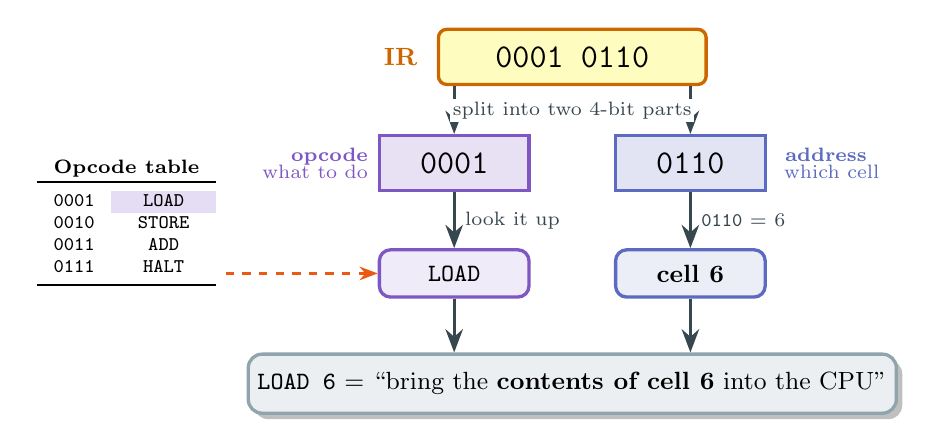
\begin{tikzpicture}[>=Stealth,
      field/.style={very thick, minimum width=1.9cm, minimum height=0.7cm, font=\ttfamily\large},
      meaning/.style={very thick, rounded corners=4pt, minimum width=1.9cm, minimum height=0.6cm,
        font=\small\bfseries, align=center},
      flow/.style={->, very thick, nInk}]
      % the instruction in the IR
      \node[draw=orange!80!black, fill=yellow!25, very thick, rounded corners=3pt, minimum width=3.4cm,
        minimum height=0.7cm, font=\ttfamily\large] (ir) at (3.5,1.9) {0001 0110};
      \node[anchor=east, font=\small\bfseries, text=orange!80!black] at (ir.west) {IR\ \ };
      % the two parts
      \node[field, draw=sViolet, fill=sViolet!18] (op) at (2.0,0.55) {0001};
      \node[field, draw=sIndigo, fill=sIndigo!18] (ad) at (5.0,0.55) {0110};
      \node[anchor=east, font=\scriptsize\bfseries, text=sViolet, align=right] at (op.west) {opcode\\[-2pt]\mdseries what to do\ };
      \node[anchor=west, font=\scriptsize\bfseries, text=sIndigo, align=left] at (ad.east) {\ address\\[-2pt]\mdseries\ which cell};
      \draw[flow] (ir.south -| op.north) -- (op.north);
      \draw[flow] (ir.south -| ad.north) -- (ad.north);
      \node[font=\scriptsize, text=nInk, fill=white, inner sep=1pt] at (3.5,1.22) {split into two 4-bit parts};
      % what each part means
      \node[meaning, draw=sViolet, fill=sViolet!12] (load) at (2.0,-0.85) {\texttt{LOAD}};
      \node[meaning, draw=sIndigo, fill=sIndigo!12] (cell) at (5.0,-0.85) {cell 6};
      \draw[flow] (op) -- node[right, font=\scriptsize] {look it up} (load);
      \draw[flow] (ad) -- node[right, font=\scriptsize] {\texttt{0110} = 6} (cell);
      % opcode table
      \node[anchor=east, font=\scriptsize] (tab) at (-0.9,-0.2) {%
        \begin{tabular}{cc}
          \multicolumn{2}{c}{\textbf{Opcode table}} \\
          \toprule
          \texttt{0001} & \cellcolor{sViolet!20}\texttt{LOAD} \\
          \texttt{0010} & \texttt{STORE} \\
          \texttt{0011} & \texttt{ADD} \\
          \texttt{0111} & \texttt{HALT} \\
          \bottomrule
        \end{tabular}};
      \draw[->, thick, dashed, AccentOrange] (tab.east |- load) -- (load.west);
      % the result
      \node[draw=nLine, very thick, rounded corners=5pt, fill=nFill, minimum width=7.2cm,
        minimum height=0.75cm, font=\small, drop shadow] (res) at (3.5,-2.25)
        {\texttt{LOAD 6} = ``bring the \textbf{contents of cell 6} into the CPU''};
      \draw[flow] (load.south) -- (load.south |- res.north);
      \draw[flow] (cell.south) -- (cell.south |- res.north);
    \end{tikzpicture}
  \end{center}
  \vfill
  \phasename{decode}
  \vspace{0.05cm}
\end{frame}

% ---------- 5. Execute: AC ----------
\explainframe{The accumulator (AC) and execute}
  {\mempanel{-1}{0000 0000\ \ (0)}{6}
   \cpupanel{3}{1}{0001 0110}{5}{}
   \executing{LOAD 6}
   \draw[dataarrow] (m6.east) -- ++(0.75,0) |- (ac.west);
   \node[steplabel, text=aRead] at (2.2,-0.62) {read};}
  {\footnotesize
   The CPU reads \textbf{cell 6}. Memory sends back \mbox{\texttt{0000 0101}} = 5.\par\vspace{0.04cm}
   \textcolor{DeepBlue}{The instruction said \textbf{6}, the value we got is \textbf{5}: 6 was the number of the cell.}\par\vspace{0.08cm}
   \defbox{The \textbf{accumulator (AC)} is a register that holds the working value:
     the number the CPU is working with right now.}
   \footnotesize
   The CPU keeps the 5 in the AC because the next instruction (\texttt{ADD 7}) will need it.\par\vspace{0.08cm}
   Nothing was calculated: \texttt{LOAD} only moves a value.\par\vspace{0.1cm}
   \phasename{execute}\vspace{0.06cm}
   \statebox{\texttt{PC = 1}, \ \texttt{IR = LOAD 6}, \ \texttt{AC = 5}}}

% ---------- 6. What did we just do? ----------
\begin{frame}{What did we just do?}
  \begin{beamercolorbox}[rounded=true,sep=0.14cm,wd=\textwidth]{block body}
    \centering\small
    One instruction took \textbf{three phases}. Now the CPU simply repeats them for the next instruction.
  \end{beamercolorbox}
  \vspace{0.3cm}
  \begin{center}
    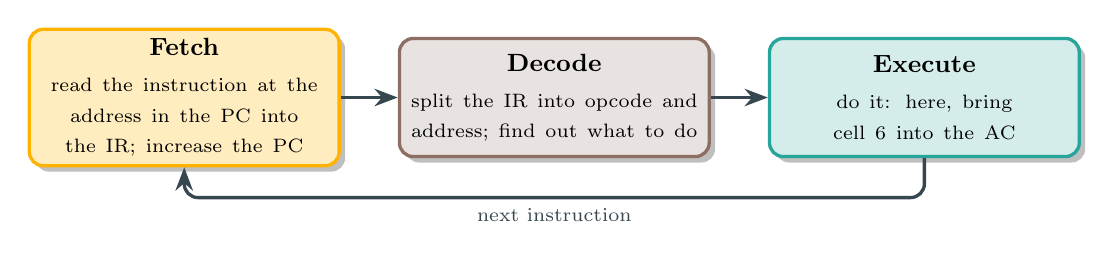
\begin{tikzpicture}[>=Stealth,
      phase/.style={very thick, rounded corners=5pt, minimum width=3.9cm, minimum height=1.5cm,
        align=center, font=\small\bfseries, drop shadow, text width=3.7cm}]
      \node[phase, draw=sAmber, fill=sAmber!25] (f) at (0,0)
        {Fetch\\[2pt]\scriptsize\mdseries read the instruction at the address in the PC into the IR; increase the PC};
      \node[phase, draw=sBrown, fill=sBrown!20] (d) at (4.7,0)
        {Decode\\[2pt]\scriptsize\mdseries split the IR into opcode and address; find out what to do};
      \node[phase, draw=sTeal, fill=sTeal!20] (e) at (9.4,0)
        {Execute\\[2pt]\scriptsize\mdseries do it: here, bring cell 6 into the AC};
      \draw[->, very thick, nInk] (f) -- (d);
      \draw[->, very thick, nInk] (d) -- (e);
      \draw[->, very thick, nInk, rounded corners=5pt] (e.south) -- ++(0,-0.5) -| (f.south)
        node[pos=0.25, below, font=\scriptsize] {next instruction};
    \end{tikzpicture}
  \end{center}
  \vfill
  \begin{beamercolorbox}[rounded=true,sep=0.12cm,wd=\textwidth]{block body example}
    \centering\footnotesize
    The PC already holds \texttt{1}, so the CPU is ready for the next instruction: \texttt{ADD 7}.
  \end{beamercolorbox}
\end{frame}

% ---------- 7. ADD 7: fetch and decode ----------
\explainframe{\texttt{ADD 7}: fetch and decode}
  {\mempanel{1}{0000 0000\ \ (0)}{0}
   \cpupanel{3}{1 $\to$ 2}{0011 0111}{5}{}
   \draw[fetcharrow] (m1.east) -- ++(0.4,0) |- (ir.west);
   \node[steplabel, text=aRead] at (1.85,0.45) {read};}
  {\stepbox{\textcolor{sAmberText}{Fetch}}{\texttt{PC = 1}: read cell 1\\
     \texttt{IR} $\leftarrow$ \mbox{\texttt{0011 0111}}\\ \texttt{PC} $\to$ 2}
   \stepbox{\textcolor{sBrown}{Decode}}{\texttt{0011} = \texttt{ADD}\\ \texttt{0111} = cell 7}
   \begin{beamercolorbox}[rounded=true,sep=0.1cm,wd=\linewidth]{block body example}
     \footnotesize\centering
     The same steps as before, only different bits.
   \end{beamercolorbox}
   \vspace{0.06cm}
   {\centering\scriptsize \texttt{ADD 7} names only one cell. The other number\\
     always comes from the AC, which still holds \texttt{5}.\par}}

% ---------- 8. ADD 7: execute, ALU ----------
\explainframe{The arithmetic logic unit (ALU)}
  {\mempanel{-1}{0000 0000\ \ (0)}{7}
   \cpupanel{4}{2}{0011 0111}{5 $\to$ 8}{hotalu}
   \executing{ADD 7}
   % input 1: from the AC
   \draw[-{Stealth}, very thick, nInk]
     ([yshift=4pt]ac.east) -- node[above, font=\tiny\bfseries] {5} ([yshift=4pt]alu.west);
   % result: back to the AC
   \draw[-{Stealth}, very thick, nInk]
     ([yshift=-4pt]alu.west) -- node[below, font=\tiny\bfseries] {8} ([yshift=-4pt]ac.east);
   % input 2: from cell 7
   \draw[dataarrow] (m7.east) -- ++(0.45,0) |- (6.3,-1.85) -- (alu.south);
   \node[font=\tiny\bfseries, text=aRead, above] at (4.1,-1.85) {3 from cell 7};}
  {\footnotesize
   \texttt{ADD 7} needs two numbers: \textbf{5} from the AC and \textbf{3} from cell 7.\par\vspace{0.15cm}
   \defbox{The CPU has a \textbf{specialised unit} for calculations:
     the \textbf{arithmetic logic unit (ALU)}.}
   \vspace{0.05cm}
   \footnotesize Both numbers go into the ALU. The result goes back to the AC.\par\vspace{0.15cm}
   \phasename{execute}\vspace{0.06cm}
   \statebox{\texttt{PC = 2}, \ \texttt{IR = ADD 7}, \ \texttt{AC = 8}}}

% ---------- 9. STORE 8 ----------
\explainframe{\texttt{STORE 8}: data goes the other way}
  {\mempanel{2}{0000 1000\ \ (8)}{8}
   \cpupanel{4}{2 $\to$ 3}{0010 1000}{8}{}
   \draw[fetcharrow] (m2.east) -- ++(0.4,0) |- (ir.west);
   \draw[dataarrow] (ac.west) -- (2.2,-1.05) |- (m8.east);
   \node[steplabel, text=aRead] at (1.85,0.22) {read};
   \node[steplabel, text=aWrite] at (2.2,-1.45) {write};}
  {\stepbox{\textcolor{sAmberText}{Fetch}}{\texttt{PC = 2}: read cell 2; \texttt{IR} $\leftarrow$ \mbox{\texttt{0010 1000}};
     \texttt{PC} $\to$ 3}
   \stepbox{\textcolor{sBrown}{Decode}}{\texttt{0010} = \texttt{STORE}; \ \texttt{1000} = cell 8}
   \stepbox{\textcolor{sTealText}{Execute}}{write the AC into cell 8:
     data goes \textbf{from the CPU to memory}.\\
     Cell 8: \mbox{\texttt{0000 0000}} $\to$ \mbox{\texttt{0000 1000}}}
   \begin{beamercolorbox}[rounded=true,sep=0.1cm,wd=\linewidth]{block body example}
     \footnotesize\centering
     The first moment the program \textbf{changes} memory.
   \end{beamercolorbox}}

% ---------- 10. HALT ----------
\explainframe{\texttt{HALT}: the end of the program}
  {\mempanel{3}{0000 1000\ \ (8)}{0}
   \cpupanel{4}{3 $\to$ 4}{0111 0000}{8}{}
   \draw[fetcharrow] (m3.east) -- ++(0.4,0) |- (ir.west);
   \node[steplabel, text=aRead] at (2.0,0.2) {read};}
  {\stepbox{\textcolor{sAmberText}{Fetch}}{\texttt{PC = 3}: read cell 3; \texttt{IR} $\leftarrow$ \mbox{\texttt{0111 0000}};
     \texttt{PC} $\to$ 4}
   \stepbox{\textcolor{sBrown}{Decode}}{\texttt{0111} = \texttt{HALT}}
   \stepbox{\textcolor{sTealText}{Execute}}{the CPU stops repeating the cycle.}
   \begin{beamercolorbox}[rounded=true,sep=0.1cm,wd=\linewidth]{block body example}
     \footnotesize\centering
     \textbf{Result:} cell 8 holds \mbox{\texttt{0000 1000}} = 8 = 5 + 3.
   \end{beamercolorbox}}

% ---------- 11. The control unit and the complete CPU ----------
\begin{frame}{Who was directing all of this?}
  \begin{beamercolorbox}[rounded=true,sep=0.14cm,wd=\textwidth]{block body}
    \centering\small
    We kept saying ``the CPU reads'', ``the CPU decodes'', ``the CPU increases the PC''.
    The part of the CPU that does these things in the right order is the \textbf{CU (control unit)}.
  \end{beamercolorbox}
  \vspace{0.1cm}
  \begin{columns}[c,onlytextwidth]
    \column{0.36\textwidth}
      \centering
      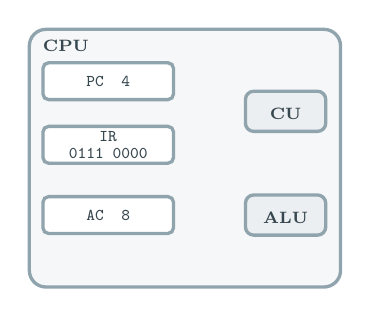
\begin{tikzpicture}[>=Stealth, scale=0.85, every node/.append style={transform shape}]
        \cpupanel{5}{4}{0111 0000}{8}{}
      \end{tikzpicture}
    \column{0.62\textwidth}
      \centering
      \scriptsize
      \renewcommand{\arraystretch}{1.2}
      \begin{tabular}{lll}
        \toprule
        \textbf{Problem} & \textbf{Solution} & \textbf{Box in Decision 5} \\
        \midrule
        Which cell to read next? & PC & \colorbox{yellow!30}{Registers} \\
        Where to keep the instruction? & IR & \colorbox{yellow!30}{Registers} \\
        What do the bits mean? & decoding & \textbf{CU} \\
        Where to keep the working value? & AC & \colorbox{yellow!30}{Registers} \\
        Who calculates? & ALU & \textbf{ALU} \\
        Who runs the whole sequence? & CU & \textbf{CU} \\
        \bottomrule
      \end{tabular}
  \end{columns}
  \vspace{0.15cm}
  \begin{columns}[T,onlytextwidth]
    \column{0.47\textwidth}
      \begin{beamercolorbox}[rounded=true,sep=0.12cm,wd=\linewidth]{block body example}
        \centering\footnotesize
        The \textbf{CU} decides and coordinates, but never calculates.
      \end{beamercolorbox}
    \column{0.47\textwidth}
      \begin{beamercolorbox}[rounded=true,sep=0.12cm,wd=\linewidth]{block body example}
        \centering\footnotesize
        The \textbf{ALU} calculates, but never decides what to do.
      \end{beamercolorbox}
  \end{columns}
\end{frame}

% ---------- 12. The instruction cycle ----------
\begin{frame}{The instruction cycle: fetch, decode, execute}
  \begin{beamercolorbox}[rounded=true,sep=0.1cm,wd=\textwidth]{block body}
    \centering\footnotesize
    What we have just seen four times, written compactly: the CPU repeats \textbf{the same three phases}
    for every instruction, until it meets \texttt{HALT}.
  \end{beamercolorbox}
  \vspace{0.06cm}
  \begin{beamercolorbox}[rounded=true,sep=0.08cm,wd=\textwidth]{block body example}
    \centering\footnotesize
    \textbf{Notation:} $\mathsf{M}[a]$ means ``the contents of memory cell number $a$'' (e.g.\ $\mathsf{M}[6] = 5$);
    \ $\leftarrow$ means ``is written into''.
  \end{beamercolorbox}
  \vspace{-0.1cm}
  \begin{center}
    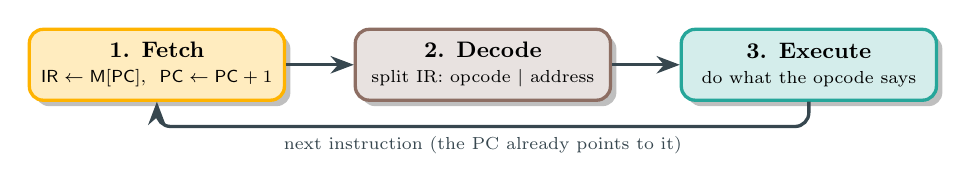
\begin{tikzpicture}[>=Stealth, scale=0.9, every node/.append style={transform shape},
      phase/.style={very thick, rounded corners=5pt, minimum width=3.6cm, minimum height=1.0cm,
        align=center, font=\small\bfseries, drop shadow}]
      \node[phase, draw=sAmber, fill=sAmber!25] (f) at (0,0)
        {1. Fetch\\[-1pt]\scriptsize\mdseries $\mathsf{IR}\leftarrow \mathsf{M}[\mathsf{PC}]$,\ \ $\mathsf{PC}\leftarrow\mathsf{PC}+1$};
      \node[phase, draw=sBrown, fill=sBrown!20] (d) at (4.6,0)
        {2. Decode\\[-1pt]\scriptsize\mdseries split IR: opcode $|$ address};
      \node[phase, draw=sTeal, fill=sTeal!20] (e) at (9.2,0)
        {3. Execute\\[-1pt]\scriptsize\mdseries do what the opcode says};
      \draw[->, very thick, nInk] (f) -- (d);
      \draw[->, very thick, nInk] (d) -- (e);
      \draw[->, very thick, nInk, rounded corners=5pt] (e.south) -- ++(0,-0.35) -| (f.south)
        node[pos=0.25, below, font=\scriptsize] {next instruction (the PC already points to it)};
    \end{tikzpicture}
  \end{center}
  \vspace{-0.2cm}
  \begin{columns}[T,onlytextwidth]
    \column{0.56\textwidth}
      \centering
      \footnotesize\textbf{What ``execute'' means for each opcode}\\[0.08cm]
      \scriptsize
      \renewcommand{\arraystretch}{1.05}
      \begin{tabular}{llp{2.5cm}}
        \toprule
        \textbf{Instruction} & \textbf{Effect} & \textbf{Needs} \\
        \midrule
        \texttt{LOAD a}  & $\mathsf{AC}\leftarrow\mathsf{M}[a]$ & read memory \\
        \texttt{ADD a}   & $\mathsf{AC}\leftarrow\mathsf{AC}+\mathsf{M}[a]$ & read memory + ALU \\
        \texttt{STORE a} & $\mathsf{M}[a]\leftarrow\mathsf{AC}$ & write memory \\
        \texttt{HALT}    & stop the cycle & nothing \\
        \bottomrule
      \end{tabular}
    \column{0.4\textwidth}
      \begin{beamercolorbox}[rounded=true,sep=0.12cm,wd=\linewidth]{block body example}
        \scriptsize
        \textbf{Fetch and decode} are identical for every instruction.
        Only \textbf{execute} differs.
      \end{beamercolorbox}
  \end{columns}
\end{frame}



% ---------- 13. The whole run ----------
\begin{frame}{The whole run in one table}
  \begin{center}
    \footnotesize\textbf{One row per instruction: which cell was read, what it meant, and the state afterwards}\\[0.12cm]
    \renewcommand{\arraystretch}{1.35}
    \begin{tabular}{ccccc}
      \toprule
      \textbf{PC (cell read)} & \textbf{Bits} & \textbf{Decoded instruction} & \textbf{AC after} & $\mathbf{M[8]}$ \textbf{after} \\
      \midrule
      0 & \mbox{\texttt{0001 0110}} & \texttt{LOAD 6}  & 5 & 0 \\
      1 & \mbox{\texttt{0011 0111}} & \texttt{ADD 7}   & 8 & 0 \\
      2 & \mbox{\texttt{0010 1000}} & \texttt{STORE 8} & 8 & 8 \\
      3 & \mbox{\texttt{0111 0000}} & \texttt{HALT}    & 8 & 8 \\
      \bottomrule
    \end{tabular}
  \end{center}
  \vspace{0.2cm}
  \begin{beamercolorbox}[rounded=true,sep=0.12cm,wd=\textwidth]{block body example}
    \centering\small
    \textbf{Result:} when the CPU stops, $\mathsf{M}[8] = 8 = 5 + 3$.
  \end{beamercolorbox}
\end{frame}

% ---------- 14. Student task: be the CPU ----------
\begin{frame}{Task: you are the CPU}
  \begin{beamercolorbox}[rounded=true,sep=0.12cm,wd=\textwidth]{block body}
    \centering\small
    \textbf{Individual task (12 min).} The memory below holds a program and its data, exactly as the CPU sees it.
    Fetch, decode and execute it by hand.
  \end{beamercolorbox}
  \vspace{0.12cm}
  \begin{columns}[T,onlytextwidth]
    \column{0.2\textwidth}
      \centering
      \footnotesize\textbf{Memory}\\[0.05cm]
      \scriptsize
      \renewcommand{\arraystretch}{1.1}
      \begin{tabular}{c|c}
        \toprule
        \textbf{Addr} & \textbf{Bits} \\
        \midrule
        0 & \mbox{\texttt{0001 0110}} \\
        1 & \mbox{\texttt{0011 0111}} \\
        2 & \mbox{\texttt{0011 0110}} \\
        3 & \mbox{\texttt{0010 1000}} \\
        4 & \mbox{\texttt{0111 0000}} \\
        5 & \mbox{\texttt{0000 0000}} \\
        6 & \mbox{\texttt{0000 0100}} \\
        7 & \mbox{\texttt{0000 1001}} \\
        8 & \mbox{\texttt{0000 0000}} \\
        \bottomrule
      \end{tabular}
    \column{0.22\textwidth}
      \centering
      \footnotesize\textbf{Opcode table}\\[0.05cm]
      \scriptsize
      \renewcommand{\arraystretch}{1.1}
      \begin{tabular}{cc}
        \toprule
        \textbf{Opcode} & \textbf{Instruction} \\
        \midrule
        \texttt{0001} & \texttt{LOAD a} \\
        \texttt{0010} & \texttt{STORE a} \\
        \texttt{0011} & \texttt{ADD a} \\
        \texttt{0111} & \texttt{HALT} \\
        \bottomrule
      \end{tabular}\\[0.08cm]
      \tiny first 4 bits = opcode,\\ last 4 bits = address \texttt{a}\\[0.15cm]
      \begin{beamercolorbox}[rounded=true,sep=0.08cm,wd=\linewidth]{block body example}
        \centering\scriptsize
        At the start \texttt{PC = 0}:\\ the program starts at cell 0.
      \end{beamercolorbox}
    \column{0.54\textwidth}
      \centering
      \footnotesize\textbf{Fill in one row per instruction}\\[0.05cm]
      \scriptsize
      \renewcommand{\arraystretch}{1.45}
      \begin{tabular}{|>{\centering\arraybackslash}p{0.95cm}|>{\centering\arraybackslash}p{1.35cm}|>{\centering\arraybackslash}p{1.5cm}|>{\centering\arraybackslash}p{0.9cm}|>{\centering\arraybackslash}p{0.9cm}|}
        \hline
        \textbf{PC (cell read)} & \textbf{Bits} & \textbf{Decoded instruction} & \textbf{AC after} & $\mathbf{M[8]}$ \textbf{after} \\
        \hline
        0 & & & & \\ \hline
          & & & & \\ \hline
          & & & & \\ \hline
          & & & & \\ \hline
          & & & & \\ \hline
      \end{tabular}
  \end{columns}
  \vfill
  \begin{beamercolorbox}[rounded=true,sep=0.1cm,wd=\textwidth]{block body example}
    \footnotesize
    \textbf{Then answer:} (a) What is in $\mathsf{M}[8]$ when the CPU stops? Give it in decimal and in binary.
    \ (b) \emph{Bonus:} what would happen if the PC ever reached address 6?
  \end{beamercolorbox}
\end{frame}

% ---------- 15. Solution ----------
\begin{frame}{Task: solution}
  \begin{columns}[T,onlytextwidth]
    \column{0.56\textwidth}
      \centering
      \scriptsize
      \renewcommand{\arraystretch}{1.35}
      \begin{tabular}{ccccc}
        \toprule
        \textbf{PC (cell read)} & \textbf{Bits} & \textbf{Decoded} & \textbf{AC after} & $\mathbf{M[8]}$ \textbf{after} \\
        \midrule
        0 & \mbox{\texttt{0001 0110}} & \texttt{LOAD 6}  & 4  & 0 \\
        1 & \mbox{\texttt{0011 0111}} & \texttt{ADD 7}   & 13 & 0 \\
        2 & \mbox{\texttt{0011 0110}} & \texttt{ADD 6}   & 17 & 0 \\
        3 & \mbox{\texttt{0010 1000}} & \texttt{STORE 8} & 17 & 17 \\
        4 & \mbox{\texttt{0111 0000}} & \texttt{HALT}    & 17 & 17 \\
        \bottomrule
      \end{tabular}
    \column{0.41\textwidth}
      \footnotesize
      \begin{beamercolorbox}[rounded=true,sep=0.1cm,wd=\linewidth]{block body}
        \textbf{(a)} $\mathsf{M}[8] = 17$ = \mbox{\texttt{0001 0001}}\\
        \scriptsize ($4 + 9 + 4$: cell 6 holds 4, cell 7 holds 9)
      \end{beamercolorbox}
      \vspace{0.08cm}
      \begin{beamercolorbox}[rounded=true,sep=0.1cm,wd=\linewidth]{block body example}
        \textbf{(b)} The CPU would fetch \mbox{\texttt{0000 0100}} and try to decode it as an instruction.
        Opcode \texttt{0000} is not in the table: a real CPU reports an \emph{illegal instruction}.
        The bits mean ``number 4'' only because the program uses them as data.
      \end{beamercolorbox}
  \end{columns}
  \vspace{0.15cm}
  \begin{beamercolorbox}[rounded=true,sep=0.1cm,wd=\textwidth]{block body}
    \centering\scriptsize
    \textbf{Typical mistakes:} using the address as the value (\texttt{ADD 6} adds the contents of cell 6, which is 4, not 6);
    reading the opcode from the wrong half; writing to $\mathsf{M}[8]$ before \texttt{STORE};
    continuing after \texttt{HALT}.
  \end{beamercolorbox}
\end{frame}

% =====================================================================
%  HANDS-ON: MARIE
% =====================================================================

\section{Programming a simple CPU}

% ---------- M1. MARIE ----------
\begin{frame}{Now a simulator is the CPU: MARIE}
  \begin{beamercolorbox}[rounded=true,sep=0.14cm,wd=\textwidth]{block body}
    \centering\small
    \textbf{MARIE} is a small CPU simulator designed for teaching. It has memory, registers,
    an accumulator, and the same fetch--decode--execute cycle we have just followed.\\[0.05cm]
    \textcolor{DeepBlue}{\faLaptop}\ \ \textbf{\url{https://marie.js.org}}\ \ (runs in the browser, nothing to install)
  \end{beamercolorbox}
  \vspace{0.3cm}
  \begin{columns}[T,onlytextwidth]
    \column{0.43\textwidth}
      \centering
      \footnotesize\textbf{From a program instruction to machine code}\\[0.12cm]
      \texttt{Load X}\\[0.08cm]
      $\Downarrow$\\[0.08cm]
      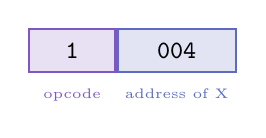
\begin{tikzpicture}
        \node[draw=sViolet, fill=sViolet!18, thick, minimum width=1.1cm, minimum height=0.55cm,
          font=\ttfamily\small] (op) {1};
        \node[draw=sIndigo, fill=sIndigo!18, thick, minimum width=1.5cm, minimum height=0.55cm,
          font=\ttfamily\small, right=0pt of op] (addr) {004};
        \node[font=\tiny, text=sViolet, below=2pt of op] {opcode};
        \node[font=\tiny, text=sIndigo, below=2pt of addr] {address of X};
      \end{tikzpicture}\\[0.15cm]
      \texttt{1004}
    \column{0.52\textwidth}
      \begin{beamercolorbox}[rounded=true,sep=0.13cm,wd=\linewidth]{block body example}
        \small
        \textbf{What the opcode does}\\[0.06cm]
        The opcode tells MARIE \textbf{what operation to perform}. The remaining part identifies the operand or address.\\[0.06cm]
        \footnotesize MARIE uses \textbf{16-bit} words: a 4-bit opcode and a 12-bit address, shown as 4 hexadecimal digits.
      \end{beamercolorbox}
      \vspace{0.1cm}
      \begin{beamercolorbox}[rounded=true,sep=0.13cm,wd=\linewidth]{block body}
        \footnotesize
        The simulator lets us observe the instruction, registers, memory, and output while the program runs.
      \end{beamercolorbox}
  \end{columns}
\end{frame}

% ---------- M2. Using MARIE.js ----------
\begin{frame}{Using MARIE.js}
  \begin{columns}[T,onlytextwidth]
    \column{0.48\textwidth}
      \footnotesize\textbf{Four steps}\\[0.1cm]
      \stepbox{1. Write}{Type the program in the code editor.}
      \stepbox{2. Assemble}{The assembler translates it into machine code and puts it in memory.}
      \stepbox{3. Step}{Execute \textbf{one instruction} and look at the registers and memory.}
      \stepbox{4. Run}{Execute the whole program until \texttt{Halt}.}
    \column{0.48\textwidth}
      \footnotesize\textbf{What you will see}\\[0.1cm]
      \begin{beamercolorbox}[rounded=true,sep=0.1cm,wd=\linewidth]{block body example}
        \footnotesize
        \textbf{AC, PC, IR}: the registers you already know.\\
        \textbf{MAR, MBR}: address and data of the current memory access; \textbf{InREG, OutREG}: input and output.
      \end{beamercolorbox}
      \vspace{0.06cm}
      \begin{beamercolorbox}[rounded=true,sep=0.1cm,wd=\linewidth]{block body}
        \footnotesize
        \textbf{Memory view}: every cell in hexadecimal.\\
        \textbf{Output}: values printed by the program.
      \end{beamercolorbox}
      \vspace{0.06cm}
      {\centering\scriptsize\textcolor{DeepBlue}{Tip: choose \textbf{DEC} (decimal) for input and output.}\par}
  \end{columns}
\end{frame}

% ---------- M3. Exercise 1 ----------
\begin{frame}[fragile]{Exercise 1: our program in MARIE}
  \begin{columns}[T,onlytextwidth]
    \column{0.4\textwidth}
\begin{lstlisting}[style=marie]
Load X     / AC <- M[X]
Add Y      / AC <- AC + M[Y]
Store Z    / M[Z] <- AC
Halt
X, DEC 5   / data
Y, DEC 3
Z, DEC 0
\end{lstlisting}
      \vspace{0.05cm}
      \scriptsize
      Line number = memory address.\\
      \texttt{X, DEC 5}: cell named \texttt{X} holding the decimal value 5.\\
      Text after \texttt{/} is a comment.
    \column{0.57\textwidth}
      \begin{beamercolorbox}[rounded=true,sep=0.12cm,wd=\linewidth]{block body example}
        \small\textbf{Explore the program in MARIE}\\[0.05cm]
        \footnotesize Type the program and click \textbf{Assemble}.
      \end{beamercolorbox}
      \vspace{0.1cm}
      \footnotesize
      \begin{enumerate}\setlength{\itemsep}{3pt}
        \item Look at the Memory browser. In which memory cells are \texttt{Load X},
          \texttt{Add Y}, \texttt{Store Z} and \texttt{Halt}?
        \item What is stored in memory cells 4, 5 and 6?
        \item Click \textbf{Step} once. Notice that \textbf{AC} changes from \texttt{0000}
          to \texttt{0005}. Why?
        \item Click \textbf{Step} again. What is the value of \textbf{AC} now, and why does it have this value?
        \item Memory cell 6 still contains \texttt{0000}. Click \textbf{Step} once more.
          What value does cell 6 contain now, and why did it change?
      \end{enumerate}
  \end{columns}
\end{frame}

\begin{frame}{Solution: exercise 1}
  \begin{columns}[T,onlytextwidth]
    \column{0.5\textwidth}
      \centering
      \footnotesize\textbf{Memory after Assemble}\\[0.08cm]
      \scriptsize
      \renewcommand{\arraystretch}{1.2}
      \begin{tabular}{ccl}
        \toprule
        \textbf{Address} & \textbf{Contents} & \textbf{Meaning} \\
        \midrule
        0 & \texttt{1004} & \texttt{Load X} \\
        1 & \texttt{3005} & \texttt{Add Y} \\
        2 & \texttt{2006} & \texttt{Store Z} \\
        3 & \texttt{7000} & \texttt{Halt} \\
        4 & \texttt{0005} & \texttt{X} \\
        5 & \texttt{0003} & \texttt{Y} \\
        6 & \texttt{0000} & \texttt{Z} \\
        \bottomrule
      \end{tabular}
    \column{0.45\textwidth}
      \begin{beamercolorbox}[rounded=true,sep=0.11cm,wd=\linewidth]{block body example}
        \footnotesize
        \textbf{After the first Step:} \texttt{Load X} reads the contents of cell 4 and puts $5$ into the AC.
      \end{beamercolorbox}
      \vspace{0.08cm}
      \begin{beamercolorbox}[rounded=true,sep=0.11cm,wd=\linewidth]{block body}
        \footnotesize
        \textbf{After the second Step:} \texttt{Add Y} reads cell 5 and adds $3$ to the AC: $5+3=8$.
      \end{beamercolorbox}
      \vspace{0.08cm}
      \begin{beamercolorbox}[rounded=true,sep=0.11cm,wd=\linewidth]{block body example}
        \footnotesize
        \textbf{After the third Step:} \texttt{Store Z} writes $8$ into cell 6. The program remains in cells 0--3.
      \end{beamercolorbox}
  \end{columns}
\end{frame}

% ---------- M4. New instructions: Subt, Input, Output ----------
\begin{frame}[fragile]{New instructions: Subt, Input, Output}
  \begin{center}
    \scriptsize
    \renewcommand{\arraystretch}{1.08}
    \begin{tabular}{llcl}
      \toprule
      \textbf{Instruction} & \textbf{Effect} & \textbf{Opcode} & \textbf{In words} \\
      \midrule
      \rowcolor{LightGray}\texttt{Load X}  & $\mathsf{AC}\leftarrow\mathsf{M}[X]$ & 1 & bring the contents of \texttt{X} into the AC \\
      \rowcolor{LightGray}\texttt{Store X} & $\mathsf{M}[X]\leftarrow\mathsf{AC}$ & 2 & write the AC into \texttt{X} \\
      \rowcolor{LightGray}\texttt{Add X}   & $\mathsf{AC}\leftarrow\mathsf{AC}+\mathsf{M}[X]$ & 3 & add the contents of \texttt{X} to the AC \\
      \texttt{Subt X}  & $\mathsf{AC}\leftarrow\mathsf{AC}-\mathsf{M}[X]$ & 4 & \textbf{subtract} the contents of \texttt{X} from the AC \\
      \texttt{Input}   & $\mathsf{AC}\leftarrow$ value typed by the user & 5 & \textbf{read} a number from the user \\
      \texttt{Output}  & show the AC & 6 & \textbf{print} the value in the AC \\
      \rowcolor{LightGray}\texttt{Halt}    & stop & 7 & end of the program \\
      \bottomrule
    \end{tabular}\\[0.05cm]
    \scriptsize\textcolor{gray}{grey rows: instructions you already know}
  \end{center}
  \vspace{0.05cm}
  \begin{columns}[T,onlytextwidth]
    \column{0.42\textwidth}
\begin{lstlisting}[style=marie]
Input      / read a number
Subt One   / AC <- AC - 1
Output     / print it
Halt
One, DEC 1
\end{lstlisting}
    \column{0.55\textwidth}
      \begin{beamercolorbox}[rounded=true,sep=0.1cm,wd=\linewidth]{block body}
        \footnotesize
        \textbf{Example:} prints the number typed by the user, minus 1.
        MARIE has no ``subtract 1'' instruction, so we keep the value 1 in a cell named \texttt{One}.
      \end{beamercolorbox}
  \end{columns}
\end{frame}

% ---------- M5. Exercise 2 ----------
\begin{frame}{Exercise 2: sum two inputs}
  \begin{beamercolorbox}[rounded=true,sep=0.14cm,wd=0.68\textwidth]{block body example}
    \small\textbf{Task}\\[0.08cm]
    \footnotesize Read two numbers from the user and print their sum.\\[0.08cm]
    \scriptsize Test: $7$ and $5$ $\to$ $12$
  \end{beamercolorbox}
  \vspace{0.12cm}
  \begin{beamercolorbox}[rounded=true,sep=0.12cm,wd=0.68\textwidth]{block body}
    \footnotesize
    \textbf{Hint:} the AC holds only one value. Store the first input before reading the second one.
    Every variable needs a memory cell, for example \texttt{A, DEC 0}.
  \end{beamercolorbox}
\end{frame}

\begin{frame}[fragile]{Solution: exercise 2}
  \begin{columns}[T,onlytextwidth]
    \column{0.42\textwidth}
\begin{lstlisting}[style=marie]
Input
Store A
Input
Add A
Output
Halt
A, DEC 0
\end{lstlisting}
    \column{0.52\textwidth}
      \begin{beamercolorbox}[rounded=true,sep=0.12cm,wd=\linewidth]{block body example}
        \footnotesize
        For inputs $7$ and $5$:\\[0.04cm]
        first input: $AC=7$, then \texttt{Store A};\\
        second input: $AC=5$;\\
        \texttt{Add A}: $AC=5+7=12$.
      \end{beamercolorbox}
  \end{columns}
\end{frame}

% ---------- M5b. Exercise 3 ----------
\begin{frame}{Exercise 3: calculate $2x-y$}
  \begin{beamercolorbox}[rounded=true,sep=0.14cm,wd=0.68\textwidth]{block body example}
    \small\textbf{Task}\\[0.08cm]
    \footnotesize Read $x$ and then $y$ from the user and print $2x-y$.\\[0.08cm]
    \scriptsize Test: $x=10$, $y=3$ $\to$ $17$
  \end{beamercolorbox}
  \vspace{0.12cm}
  \begin{beamercolorbox}[rounded=true,sep=0.12cm,wd=0.68\textwidth]{block body}
    \footnotesize
    \textbf{Hint:} save both inputs. There is no multiplication instruction, so calculate $2x$ as $x+x$.
  \end{beamercolorbox}
\end{frame}

\begin{frame}[fragile]{Solution: exercise 3}
  \begin{columns}[T,onlytextwidth]
    \column{0.42\textwidth}
\begin{lstlisting}[style=marie]
Input
Store X
Input
Store Y
Load X
Add X
Subt Y
Output
Halt
X, DEC 0
Y, DEC 0
\end{lstlisting}
    \column{0.52\textwidth}
      \begin{beamercolorbox}[rounded=true,sep=0.12cm,wd=\linewidth]{block body example}
        \footnotesize
        For $x=10$, $y=3$:\\[0.04cm]
        \texttt{Load X}; \texttt{Add X}: $AC=20$;\\
        \texttt{Subt Y}: $AC=20-3=17$.
      \end{beamercolorbox}
  \end{columns}
\end{frame}

% ---------- M6. Jumps ----------
\begin{frame}[fragile]{New instructions: Jump and Skipcond}
  \begin{beamercolorbox}[rounded=true,sep=0.09cm,wd=\textwidth]{block body}
    \centering\footnotesize
    So far, the PC has moved to the next memory cell after each instruction.
    Now we introduce two instructions that can \textbf{change this normal flow}.
    \texttt{Jump} changes where the PC goes; \texttt{Skipcond} can skip the next instruction.
  \end{beamercolorbox}
  \vspace{0.02cm}
  \begin{center}
    \footnotesize
    \renewcommand{\arraystretch}{1.08}
    \begin{tabular}{ll}
      \toprule
      \textbf{Instruction} & \textbf{Effect} \\
      \midrule
      \texttt{Jump X}       & $\mathsf{PC}\leftarrow X$ \\
      \texttt{Skipcond 000} & skip the next instruction if AC $<0$ \\
      \texttt{Skipcond 400} & skip the next instruction if AC $=0$ \\
      \texttt{Skipcond 800} & skip the next instruction if AC $>0$ \\
      \bottomrule
    \end{tabular}
  \end{center}
  \vspace{0.08cm}
  \begin{beamercolorbox}[rounded=true,sep=0.1cm,wd=\textwidth]{block body example}
    \centering\footnotesize
    \texttt{Loop,} is a label. \texttt{Jump Loop} sends the PC back to that instruction.\\[0.04cm]
    \texttt{Skipcond} checks the AC; when the condition is true, it skips the next instruction.
    A complete example follows on the next slide.
  \end{beamercolorbox}
\end{frame}

\begin{frame}[fragile]{How the loop works: Jump and Skipcond}
  \begin{columns}[T,onlytextwidth]
    \column{0.45\textwidth}
\begin{lstlisting}[style=marie]
      Input
      Store N
Loop, Load N
      Output
      Subt One
      Store N
      Skipcond 400 / N = 0?
      Jump Loop    / no: repeat
      Halt         / yes: stop
N,    DEC 0
One,  DEC 1
\end{lstlisting}
    \column{0.5\textwidth}
      \footnotesize
      \textbf{What happens at the end of each pass?}
      \begin{enumerate}\setlength{\itemsep}{3pt}
        \item \texttt{Subt One} decreases \texttt{N} by 1.
        \item \texttt{Skipcond 400} checks whether the AC is zero.
        \item If AC is not zero, \texttt{Jump Loop} repeats the loop.
        \item If AC is zero, \texttt{Skipcond} skips \texttt{Jump Loop} and the PC reaches \texttt{Halt}.
      \end{enumerate}
      \vspace{0.05cm}
      \begin{beamercolorbox}[rounded=true,sep=0.1cm,wd=\linewidth]{block body example}
        \scriptsize
        For input $3$, the output is $3,2,1$. The loop stops when \texttt{N} becomes $0$.\\
        Works for input $\ge 1$: for $0$, \texttt{N} becomes negative and never reaches $0$.
      \end{beamercolorbox}
  \end{columns}
\end{frame}

% ---------- M7. Exercise 4 ----------
\begin{frame}{Exercise 4: a loop}
  \begin{beamercolorbox}[rounded=true,sep=0.14cm,wd=0.68\textwidth]{block body example}
    \small\textbf{Exercise 4: sum from 1 to $n$}\\[0.08cm]
    \footnotesize
    Read a number $n \ge 1$ and print $1+2+\dots+n$.\\[0.08cm]
    \scriptsize Test: $n=4$ $\to$ $10$
  \end{beamercolorbox}
  \vspace{0.1cm}
  \begin{beamercolorbox}[rounded=true,sep=0.1cm,wd=0.68\textwidth]{block body}
    \scriptsize
    \textbf{Hint:} add \texttt{N} to a running sum, decrease \texttt{N}, and use
    \texttt{Skipcond 400} to stop when it reaches 0.
  \end{beamercolorbox}
  \vfill
  \begin{beamercolorbox}[rounded=true,sep=0.1cm,wd=\textwidth]{block body}
    \centering\scriptsize
    If your program never stops, press \textbf{Stop}: check the condition in \texttt{Skipcond} and what is in the AC at that moment.
  \end{beamercolorbox}
\end{frame}

% ---------- M9. Solution 4 ----------
\begin{frame}[fragile]{Solution: exercise 4 (sum from 1 to $n$)}
  \begin{columns}[T,onlytextwidth]
    \column{0.45\textwidth}
\begin{lstlisting}[style=marie]
      Input
      Store N
Loop, Load N
      Add Sum
      Store Sum
      Load N
      Subt One
      Store N
      Skipcond 400 / N = 0?
      Jump Loop    / no: repeat
      Load Sum     / yes: print
      Output
      Halt
N,    DEC 0
One,  DEC 1
Sum,  DEC 0
\end{lstlisting}
    \column{0.52\textwidth}
      \begin{beamercolorbox}[rounded=true,sep=0.1cm,wd=\linewidth]{block body}
        \footnotesize
        \textbf{Run for $n = 4$}\\[0.05cm]
        \scriptsize
        \renewcommand{\arraystretch}{1.15}
        \begin{tabular}{cccc}
          \toprule
          \textbf{Pass} & \textbf{Sum after} & \textbf{N after} & \textbf{Skipcond 400} \\
          \midrule
          1 & 4 & 3 & AC $\neq 0$: jump back \\
          2 & 7 & 2 & AC $\neq 0$: jump back \\
          3 & 9 & 1 & AC $\neq 0$: jump back \\
          4 & 10 & 0 & AC $= 0$: skip \texttt{Jump} \\
          \bottomrule
        \end{tabular}
      \end{beamercolorbox}
      \vspace{0.1cm}
      \begin{beamercolorbox}[rounded=true,sep=0.1cm,wd=\linewidth]{block body example}
        \footnotesize
        After the fourth pass \texttt{Skipcond} skips \texttt{Jump Loop}, so the program prints $10$ and halts.
      \end{beamercolorbox}
  \end{columns}
\end{frame}

\end{document}